\documentclass[t,compress,mathserif,12pt,xcolor=dvipsnames]{beamer}
\setbeamertemplate{bibliography item}{\insertbiblabel}
\usepackage{etex}
\reserveinserts{28}
\definecolor{bleuUni}{RGB}{0, 157, 224}
\definecolor{marronUni}{RGB}{68, 58, 49}
\usecolortheme[named=bleuUni]{structure}
\usepackage[bars]{beamerthemetree} % Beamer theme v 2.2
\usepackage{multimedia}
\usepackage[utf8]{inputenc}
%\usepackage[frenchb]{babel}
\usepackage[T1]{fontenc}
\usepackage{kmath,kerkis}
\usepackage{xmpmulti}
%\usepackage{mathpazo}
%\usepackage[bitstream-charter]{mathdesign}
%\usepackage{lmodern}
\usepackage{booktabs}
\usepackage{multirow}
\usepackage{pgfplots}
\pgfplotsset{compat=newest}
\usepackage{tikz}
\usetikzlibrary{patterns, shapes, arrows}
\usepackage{mathtools}
\usepackage{listings}
\usepackage{eulervm}
\usepackage{pifont}% http://ctan.org/pkg/pifont
\newcommand{\cmark}{\ding{51}}%
\newcommand{\xmark}{\ding{55}}%
\usepackage{listings}
\usepackage{array}
\newcolumntype{L}[1]{>{\raggedright\let\newline\\\arraybackslash\hspace{0pt}}m{#1}}
\newcolumntype{C}[1]{>{\centering\let\newline\\\arraybackslash\hspace{0pt}}m{#1}}
\newcolumntype{R}[1]{>{\raggedleft\let\newline\\\arraybackslash\hspace{0pt}}m{#1}}

\lstset{
  language=C++,
  basicstyle=\tiny\ttfamily,
  numbers=left,
  numberstyle=\tiny\ttfamily,
  stepnumber=1,
  numbersep=5pt,
  backgroundcolor=\color{white},
  showspaces=false,
  showstringspaces=false,
  showtabs=false,
  frame=single,
  tabsize=2,
  captionpos=b,
  breaklines=true,
  breakatwhitespace=false,
  escapeinside={(*@}{@*)},
  identifierstyle=\ttfamily,
  keywordstyle=\color[rgb]{0,0,1},
  commentstyle=\color[rgb]{0.133,0.545,0.133},
  stringstyle=\color[rgb]{0.627,0.126,0.941},
  moredelim=[is][\underbar]{**}{**},
}

\lstdefinestyle{mycpp}
{
    language = C++,
    % numbers=left,
    % numbersep=0.3em,
    escapeinside={(*@}{@*)},
    tabsize=2,
    % basicstyle=\tiny\ttfamily,
    morekeywords = {constexpr,int8_t,int16_t,int32_t, size_t},
    % commentstyle=\color{comment-color},
}

\usepackage[backend=biber, style=ieee]{biblatex}
\addbibresource{bibli.bib}
\renewcommand\mkbibacro[1]{{\footnotesize\MakeUppercase{#1}}}

\mode<presentation>
\newcommand*\oldmacro{}%
\let\oldmacro\insertshorttitle%
\renewcommand*\insertshorttitle{%
 \oldmacro\hfill%
\insertframenumber\,/\,\inserttotalframenumber}
\setbeamertemplate{footline}[frame number]
\setbeamersize{text margin left=10pt,text margin right=10pt}
\setbeamerfont{frametitle}{size=\large}
\setbeamertemplate{frametitle}{ \nointerlineskip \begin{beamercolorbox}[wd=\paperwidth,ht=2.2ex,dp=0.5ex,left]{frametitle} \hspace*{3.1ex}\strut\bfseries\color{bleuUni!15!white}\insertframetitle\strut\par \end{beamercolorbox}}

\setbeamertemplate{bibliography item}{\insertbiblabel}
  \definecolor{bluecite}{HTML}{009DE0} 


\makeatletter
\def\beamer@andinst{\\[0.1em]}
\makeatother
%~~~~~~~~~~~~~~~~~~~~~~~~~~~~~~~~~~~~~~~~~~~~~~~~~~~~~~~~~~~
%\setbeamercovered{higly dynamic}
\usetheme{Ilmenau} % Beamer theme v 3.0
%\useoutertheme[subsection=true]{smoothbars}%Beamer Outer Theme-circles on top
\setbeamercolor{section in head/foot}{bg=marronUni}

\useinnertheme{circles} %rectangle bullet points instead of circle ones
\usepackage{beamerthemebars}
\setbeamercolor{navigation symbols dimmed}{fg=red!80!black}
\setbeamercolor{navigation symbols}{fg=red!80!black}
\setbeamertemplate{navigation symbols}{}%remove navigation symbols
%~~~~~~~~~~~~~~~~~~~~~~~~~~~~~~~~~~~~~~~~~~~~~~~~~~~~~~~~~~~~~~~~~~~~~
\title{\textbf{Décodage de codes polaires sur des architectures programmables}}
%\subtitle{algorithms et arhitecture}\hspace{10.7cm}
\author[Mathieu Léonardon\hspace{7.51cm}{mathieu.leonardon@ims-bordeaux.fr}]    {Mathieu Léonardon}
\titlegraphic{
\includegraphics[height=1cm]{logos/ims.png} \hfil %
              
\includegraphics[height=1cm]{logos/inp.PNG} \hfil %
              
\includegraphics[height=1cm]{logos/ub.png}  \hfil %
              
\includegraphics[height=1cm]{logos/poly.eps}}
\date{13 Décembre 2018}
%\pgfdeclareimage[height=.8cm]{logo_ISCAS}{index.png}
%\logo{\pgfuseimage{logo_ISCAS}\hspace{\dimexpr\paperwidth-3.55cm}\vspace{-8pt}}

\definecolor{dgreen}{rgb}{0.,0.6,0.}
\definecolor{milano}{rgb}{0.458824, 0.050980, 0.058824}
\definecolor{bahama}{rgb}{0.066667, 0.298039, 0.443137}
\definecolor{blupres}{RGB}{0, 157, 224}
\definecolor{redpres}{RGB}{204, 0, 0}

\newcommand\blfootnote[1]{%
  \begingroup
  \renewcommand\thefootnote{}\footnote{#1}%
  \addtocounter{footnote}{-1}%
  \endgroup
}

\newcommand{\RED} [1]{\textcolor{red}{\textbf{#1}}}
\newcommand{\ORANGE} [1]{\textcolor{orange}{\textbf{#1}}}
\newcommand{\GREEN} [1]{\textcolor{dgreen}{\textbf{#1}}}
\newcommand{\BLUE} [1]{\textcolor{blue}{\textbf{#1}}}

\newcommand{\MILANO} [1]{\textcolor{milano}{#1}}
\newcommand{\BAHAMA} [1]{\textcolor{bahama}{#1}}

\usepackage{textpos}
%\usepackage{stmaryrd}
\usepackage{amsbsy}
\usepackage{makecell}
%\usepackage{fourier-orns}
% \usepackage{tikz}
% \usetikzlibrary{patterns, shapes, arrows, shapes.multipart}

\usepackage{etoolbox}
\AtBeginSection[]
{
	\ifnumcomp{\value{section}}{=}{1}{}{
\begin{frame}[c]{Plan}
\centering
\tableofcontents[
  currentsection,
  currentsubsection,
]
\end{frame}
}
}
\AtBeginSubsection[]
{
	\begin{frame}[c]{}
\tableofcontents[
currentsection,
sectionstyle=show/show,
subsectionstyle=show/shaded/hide
]
	\end{frame}
}


% \defbeamertemplate*{title page}{customized}[1][]
% {
%   \usebeamerfont{title}\inserttitle\par
%   \usebeamerfont{subtitle}\usebeamercolor[fg]{subtitle}\insertsubtitle\par
%   \bigskip
%   \usebeamerfont{author}\insertauthor\par
%   \usebeamerfont{institute}\insertinstitute\par
%   \usebeamerfont{date}\insertdate\par
%   \usebeamercolor[fg]{titlegraphic}\inserttitlegraphic
% }

\bibliography{bibli}


% \includeonly{part3}

\begin{document}

\begin{frame}[c]
\titlepage
\end{frame}

%!TEX root = ./soutenance.tex


\section[Introduction]{Décodage de codes polaires}
\subsection*{Les codes correcteurs d'erreurs}

\begin{frame}[c]{Chaîne de communications numériques}
	\begin{center}
	\multiinclude[<+>][start=6,format=pdf,graphics={width=.8\textwidth}]{./fig/chaine_com}
	\end{center}
	\begin{itemize}
		\item<1-> Transmission de bits d'information
		\item<1-> Présence de perturbations
		\item<2-> Ajout de redondance
		\item<4-> Correction des erreurs
	\end{itemize}
\end{frame}

\begin{frame}[c]
	\tableofcontents[
	subsectionstyle=hide,
	]
\end{frame}

\begin{frame}
\vfill
	\begin{itemize}
		\item 1948 : Théorie de l’information (Shannon)
		\item 1950 : Codes de Hamming
		\item 1955 : Codes convolutifs
		\item 1960 : Codes BCH
		\item 1960 : Codes Reed-Solomon
		\item 1960 : \textbf{Codes LDPC (DVB,5G)}
		\item 1966 : Codes concaténés
		\item 1993 : \textbf{Turbocodes (4G)}
		\item 2008 : \textbf{Codes polaires (5G)}
	\end{itemize}
	\vfill
\end{frame}

\subsection*{Les codes polaires}
\begin{frame}[c]{Codes polaires}
	\begin{columns}[T] % align columns
		\begin{column}{.65\textwidth}
			\multiinclude[<+>][start=1,format=pdf,graphics={width=\textwidth}]{./fig/focus_polar}
		\end{column}
		\begin{column}{.35\textwidth}
		\begin{itemize}
			\item<1-> Matrice génératrice
			\item<1->$F^{\otimes n}$ ; $F=\left[\begin{smallmatrix} 1 & 0 \\ 1 & 1\end{smallmatrix}\right]$
			\item<2-> Bits gelés
			\item<3-> Mot de code : $\mathbold{x}$
			\item<4-> Graphe de factorisation
		\end{itemize}
		\end{column}

	\end{columns}

\end{frame}
\subsection*{Le décodage SC}

\begin{frame}[c]{Décodage de codes polaires}
	\multiinclude[<+>][start=1,format=pdf,graphics={width=\textwidth}]{./fig/decoder_in_chain}    
	\begin{itemize}
		\item<2> Estimations, LLR (Log-Likelihood Ratio)
		\item<2> Signe, valeur binaire la plus probable
		\item<2> Valeur absolue, fiabilité de l'information
	\end{itemize}
\end{frame}

\begin{frame}[c]{Algorithme de décodage SC}
	\begin{columns}[T] % align columns
		\begin{column}{.65\textwidth}
			\multiinclude[<+>][start=1,format=pdf,graphics={width=\textwidth}]{./fig/focus_decoder}
		\end{column}
		\begin{column}{.35\textwidth}
		\begin{itemize}
			\item<1-> $L$ : Log Likelihood Ratios (LLR)
			\item<3-> $s$ : Sommes Partielles
			\item<4-> $$f(L_a,L_b) \approx \text{sign}(L_a.L_b).\min(|L_a|,|L_b|)$$
			\item<5-> $$g(L_a,L_b,\hat{s}_a) = (1-2\hat{s}_a)L_a+L_b$$
		\end{itemize}
		\end{column}
	\end{columns}

\end{frame}

% \begin{frame}[c]{Algorithme de décodage SC}
% 	\begin{columns}[T] % align columns
% 		\begin{column}{.35\textwidth}
% 			\multiinclude[<+>][start=1,format=pdf,graphics={width=\textwidth}]{./fig/polar_functions}    
% 		\end{column}

% 		\begin{column}{.65\textwidth}
% 		\only<1>{
% 		$$f(L_a,L_b) \approx \text{sign}(L_a.L_b).\min(|L_a|,|L_b|)$$
% 		\vspace{1.1cm}

% 		$$g(L_a,L_b,\hat{s}_a) = (1-2\hat{s}_a)L_a+L_b$$
% 		}

% 				\only<2>{
% 				\vspace{0.5cm}
% 		$$\texttt{R1}(L_a)  =  \left\{\begin{array}{l c l} 0 \text{ si } L_a \geq 0 \\ 1 \text{ si } L_a < 0 \end{array}\right.$$
% 		\vspace{1.1cm}

% 		$$h(\hat{s}_a,\hat{s}_b) = (\hat{s}_{a} \oplus \hat{s}_{b}, \hat{s}_{b})$$
% 		}
% 		\end{column}

% 	\end{columns}

	
 %    g(L_a,L_b,\hat{s}_a)&=&(1-2\hat{s}_a)L_a+L_b\\
 %    h(\hat{s}_a,\hat{s}_b)&=& (\hat{s}_{a} \oplus \hat{s}_{b}, \hat{s}_{b})\\
 %    \texttt{R0}(L_a) &=& 0 \\
 %    \texttt{R1}(L_a) &=&  \left\{\begin{array}{l c l} 0 \text{ si } L_a \geq 0 \\ 1 \text{ si } L_a < 0 \end{array}\right.
% \end{frame}

% \begin{frame}[c]{Algorithme de décodage SC}
% 	\multiinclude[<+>][start=3,format=pdf,graphics={width=.8\textwidth}]{./fig/focus_decoder}
% \end{frame}

\begin{frame}[c]{Algorithme de décodage SC}
	\begin{columns}[T] % align columns

		\begin{column}{.55\textwidth}
			\multiinclude[<+>][start=2,format=pdf,graphics={width=\textwidth}]{./fig/sc_tree}

		\end{column}

		\begin{column}{.45\textwidth}
		\only<8>{
			\begin{itemize}
				\item \GREEN{Récursif}
				\item \GREEN{Régulier}
				\item \GREEN{Atteint la capacité pour une taille de mot de code infinie}
				\vspace{0.5cm}
				\item \RED{Performances faibles pour $N<4096$}
				\item \RED{Problème de propagation des erreurs}
			\end{itemize}
		}
		\end{column}

	\end{columns}

\end{frame}


\subsection*{Le décodage SC Liste}

\begin{frame}[c]{}
  	\frametitle<1-7>{Algorithme de décodage SCL}
  	\frametitle<8->{Algorithme de décodage CASCL}
	\begin{columns}[T] % align columns

		\begin{column}{.7\textwidth}

			\multiinclude[<+>][start=1,format=pdf,graphics={width=\textwidth}]{./fig/scl_anim}

		\end{column}
\only<1-7>
 {
		\begin{column}{.3\textwidth}
			\begin{itemize}
				\item<3-7> Pas de décision dure
				\item<4-7> Duplication des candidats
				\item<5-7> Métrique de candidats
				\item<6-7> Tri des métrique \& élimination
				\item<7-7> Mot de code décodé
			\end{itemize}
		\end{column}
}
\only<8->
 {
		\begin{column}{.3\textwidth}
			\begin{itemize}
				\item<8-> Concaténation d'un CRC
				\item<9-> Utilisé pour discriminer les candidats
			\end{itemize}
		\end{column}
}
	\end{columns}
\end{frame}


\begin{frame}[c]{Performances de décodage}
	\centering
	\multiinclude[<+>][start=1,format=pdf,graphics={width=0.9\textwidth}]{./fig/scl_L/tikz/source}
\end{frame}

\begin{frame}[c]{\'Elagage de l'arbre}
			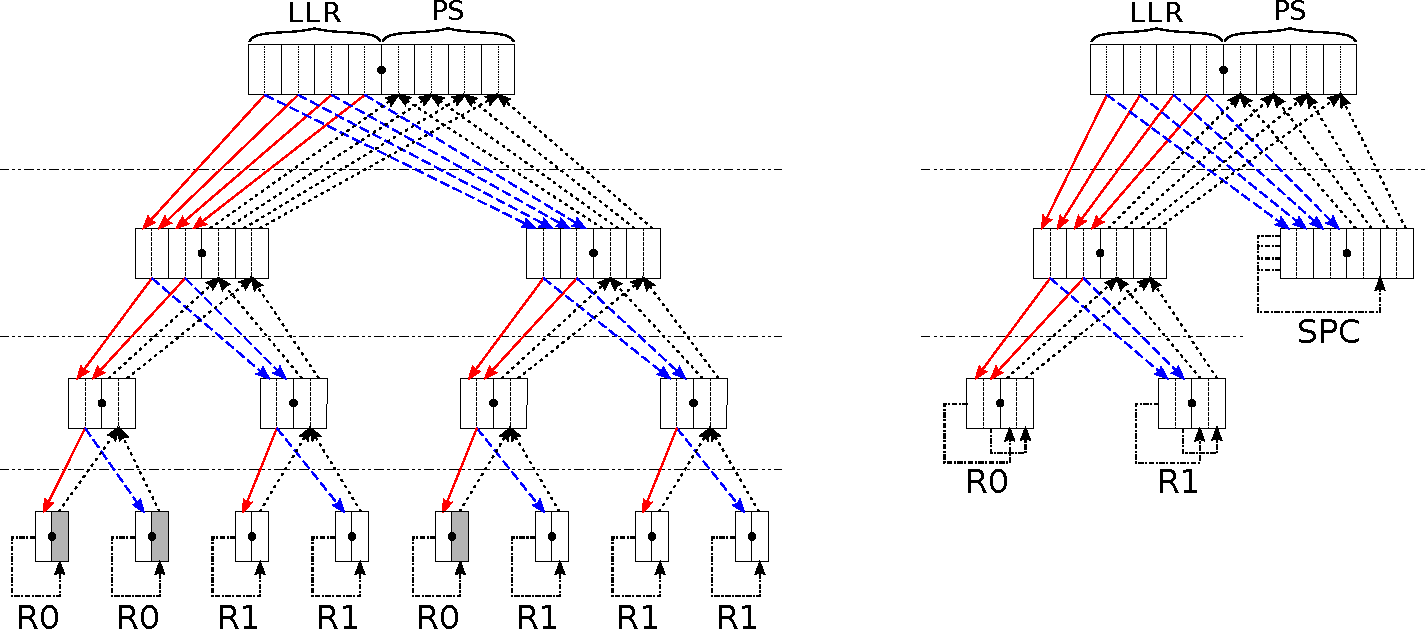
\includegraphics[width=\textwidth]{./fig/pruning}
\end{frame}
	
	\begin{frame}[c]{Résumé}
	\vspace{-0.5cm}
	\begin{minipage}[t][2cm][t]{\textwidth}
		\begin{itemize}
			\item<+-> Rôle des codes correcteurs d'erreurs
			\item<+-> Les codes polaires
			\item<+-> Compromis entre performances de décodage, débit et latence
		\end{itemize}
	\end{minipage}
	\vspace{0.5cm}	
	\begin{minipage}[t][2cm][t]{\textwidth}
	\only<3>{
		\begin{table}[t]
			\centering
			{\small\resizebox{0.8\linewidth}{!}{
			\begin{tabular}{r|c|c|c} 
				\textbf{Algorithme}  & \textbf{Performances}  & \multirow{2}{*}{\textbf{Débit}} & \textbf{Latence}  \\
				\textbf{de décodage} & \textbf{BER \& FER}    &                                 & \textbf{Maximum}  \\
				\hline
				SC           & \RED{faibles}                  & \GREEN{haut}                    & \GREEN{faible}    \\
				SCL          & \ORANGE{moyennes}              & \RED{bas}                       & \ORANGE{moyenne}  \\
				CASCL       & \GREEN{élevées}            & \RED{bas}                       & \ORANGE{moyenne}  \\
				PASCL       & \GREEN{élevées}            & \GREEN{haut}                    & \ORANGE{moyenne}       \\
				FASCL       & \GREEN{élevées}            & \GREEN{haut}                    & \RED{forte}       \\
			\end{tabular}
			}}
		\end{table}
	}
	\end{minipage}

\end{frame}
%!TEX root = ./soutenance.tex
\section[Décodeur logiciel à liste]{Décodage à liste sur processeurs généralistes}
\subsection*{}

\begin{frame}[c]{\'Evolutions des systèmes de télécommunications}
	\multiinclude[<+>][start=4,format=pdf,graphics={width=\textwidth}]{./fig/bs_evo}
	\begin{itemize}
		\item Architectures dédiées à distance pour le calcul bande de base
		\item Décodeurs logiciels
		\item Adaptativité de l'infrastructure
	\end{itemize}
\end{frame}

% \begin{frame}[c]{Décodeur logiciel}
% 	\begin{itemize}
% 		\vfill
% 		\item Architecture x86-64 majoritaire dans les serveurs
%     \vfill
%     \item Description logicielle du décodeur
%     \vfill
%     \item Exploiter les unités SIMD
% 		\vfill
% 		\item Meilleure efficacité énergétique : ARM
% 		\vfill
% 	\end{itemize}
% \end{frame}

\begin{frame}[c]{Généricité et Flexibilité d'un décodeur}
  \vfill
	\begin{itemize}
		\item Généricité : capacité à s'adapter au schéma de codage
		\begin{itemize}
			\item N, K
			\item Concaténation de CRC
			\item Position des bits gelés
			\item Poinçonnage
		\end{itemize}
    \vfill
		\item Flexibilité : capacité à supporter différentes techniques de décodages
		\begin{itemize}
			\item Variantes algorithmiques
			\item Taille de la liste
			\item Représentation en virgule fixe
			\item Ajustement de l'élagage
		\end{itemize}
	\end{itemize}
  \vfill
\end{frame}


\begin{frame}[c]{Généricité et Flexibilité d'un décodeur}
    \centering

  \renewcommand*{\thefootnote}{\alph{footnote}}
  \begin{table}[t]
    {\small\resizebox{0.8\linewidth}{!}{
      \begin{tabular}{r|C{1.5cm}C{1.5cm}C{1.5cm}C{2cm}} 
       Décodeur     & \cite{shen_low-latency_2016} & \cite{sarkis_increasing_2014} & \cite{sarkis_fast_2016} & Ce travail  \\
      \cmidrule(lr){1-1}
      \cmidrule(lr){2-2}
      \cmidrule(lr){3-3}
      \cmidrule(lr){4-4}
      \cmidrule(lr){5-5}
       N               & \GREEN{\cmark}            & \GREEN{\cmark}                & \GREEN{\cmark}          & \GREEN{\cmark} \\
       K               & \GREEN{\cmark}            & \GREEN{\cmark}                & \GREEN{\cmark}          & \GREEN{\cmark} \\
       CRC             & \GREEN{\cmark}            & \GREEN{\cmark}                & \GREEN{\cmark}          & \GREEN{\cmark} \\
       Pos. bits gelés & \GREEN{\cmark}            & \GREEN{\cmark}                & \GREEN{\cmark}          & \GREEN{\cmark} \\
       Poinçonnage  & \xmark                       & \xmark                        & \xmark                  & \cmark \\
       \hline
       PASCL        & \xmark                       & \cmark                        & \cmark                  & \cmark \\
       FASCL        & \xmark                       & \xmark                        & \xmark                  & \cmark \\
       Virgule fixe & \xmark                       & \xmark                        & \xmark                  & \cmark \\
       \'Elagage    & Statique                         &  Statique                           &  Statique                     & Dynamique \\
       Code déroulé & NON                  & NON                   & OUI               & NON \\
       % Code déroulé & \GREEN{NON}                  & \GREEN{NON}                   & \RED{OUI}               & \GREEN{NON} \\

      \end{tabular}
    }}
  \end{table}


\end{frame}


\begin{frame}[c]{Généricité et Flexibilité d'un décodeur}
    \centering

  \renewcommand*{\thefootnote}{\alph{footnote}}
      \only<1>{
      \begin{table}[t]
    {\small\resizebox{0.8\linewidth}{!}{
      \begin{tabular}{r|C{1.5cm}C{1.5cm}C{1.5cm}C{2cm}} 
       Décodeur     & \cite{shen_low-latency_2016} & \cite{sarkis_increasing_2014} & \cite{sarkis_fast_2016} & Ce travail  \\
      \cmidrule(lr){1-1}
      \cmidrule(lr){2-2}
      \cmidrule(lr){3-3}
      \cmidrule(lr){4-4}
      \cmidrule(lr){5-5}
       Poinçonnage  & {\xmark}                       & {\xmark}                        & {\xmark}                  & {\cmark} \\
       PASCL        & {\xmark}                       & {\cmark}                        & {\cmark}                  & {\cmark} \\
       FASCL        & {\xmark}                        & {\xmark}                        & {\xmark}                  & {\cmark} \\
       Virgule fixe & \xmark                       & \xmark                        & \xmark                  & \cmark \\
       \'Elagage    & Statique                         &  Statique                           &  Statique                     & Dynamique \\
       Latence ($\mu s$)\footnotemark[1]      &     1572  \footnotemark[2]                        & 3300  \footnotemark[3]                      & 433 \footnotemark[3]                 & 770 \footnotemark[3]\\
       Code déroulé & NON                  & NON                   & OUI               & NON \\
       % Code déroulé & \GREEN{NON}                  & \GREEN{NON}                   & \RED{OUI}               & \GREEN{NON} \\

      \end{tabular}
    }}
  \end{table}
  }    
  \only<2>{
      \begin{table}[t]
    {\small\resizebox{0.8\linewidth}{!}{
      \begin{tabular}{r|C{1.5cm}C{1.5cm}C{1.5cm}C{2cm}} 
       Décodeur     & \cite{shen_low-latency_2016} & \cite{sarkis_increasing_2014} & \cite{sarkis_fast_2016} & Ce travail  \\
      \cmidrule(lr){1-1}
      \cmidrule(lr){2-2}
      \cmidrule(lr){3-3}
      \cmidrule(lr){4-4}
      \cmidrule(lr){5-5}
       Poinçonnage  & \RED{\xmark}                       & \RED{\xmark}                        & \RED{\xmark}                  & \GREEN{\cmark} \\
       PASCL        & {\xmark}                       & {\cmark}                        & {\cmark}                  & {\cmark} \\
       FASCL        & {\xmark}                        & {\xmark}                        & {\xmark}                  & {\cmark} \\
       Virgule fixe & \xmark                       & \xmark                        & \xmark                  & \cmark \\
       \'Elagage    & Statique                         &  Statique                           &  Statique                     & Dynamique \\
       Latence ($\mu s$)\footnotemark[1]      &     1572  \footnotemark[2]                        & 3300  \footnotemark[3]                      & 433 \footnotemark[3]                 & 770 \footnotemark[3]\\
       Code déroulé & NON                  & NON                   & OUI               & NON \\
       % Code déroulé & \GREEN{NON}                  & \GREEN{NON}                   & \RED{OUI}               & \GREEN{NON} \\

      \end{tabular}
    }}
  \end{table}
  }    
  \only<3>{
      \begin{table}[t]
    {\small\resizebox{0.8\linewidth}{!}{
      \begin{tabular}{r|C{1.5cm}C{1.5cm}C{1.5cm}C{2cm}} 
       Décodeur     & \cite{shen_low-latency_2016} & \cite{sarkis_increasing_2014} & \cite{sarkis_fast_2016} & Ce travail  \\
      \cmidrule(lr){1-1}
      \cmidrule(lr){2-2}
      \cmidrule(lr){3-3}
      \cmidrule(lr){4-4}
      \cmidrule(lr){5-5}
       Poinçonnage  & \RED{\xmark}                       & \RED{\xmark}                        & \RED{\xmark}                  & \GREEN{\cmark} \\
       PASCL        & \RED{\xmark}                       & \GREEN{\cmark}                        & \GREEN{\cmark}                  & \GREEN{\cmark} \\
       FASCL        & \RED{\xmark}                        & \RED{\xmark}                        & \RED{\xmark}                  & \GREEN{\cmark} \\
       Virgule fixe & \xmark                       & \xmark                        & \xmark                  & \cmark \\
       \'Elagage    & Statique                         &  Statique                           &  Statique                     & Dynamique \\
       Latence ($\mu s$)\footnotemark[1]      &     1572  \footnotemark[2]                        & 3300  \footnotemark[3]                      & 433 \footnotemark[3]                 & 770 \footnotemark[3]\\
       Code déroulé & NON                  & NON                   & OUI               & NON \\
       % Code déroulé & \GREEN{NON}                  & \GREEN{NON}                   & \RED{OUI}               & \GREEN{NON} \\

      \end{tabular}
    }}
  \end{table}
  }
  \footnotetext[1]{CRC-SCL, $K=1723$, $N=2048$} 
  \footnotetext[2]{Processeur Intel i7-4790K}
  \footnotetext[3]{Processeur Intel i7-2600} 
\end{frame}

\begin{frame}
\vfill
	\only<1>{
    \begin{table}[ht]
      \centering
      {\small\resizebox{0.8\linewidth}{!}{
      \begin{tabular}{r|c|c|c c c}
         \multirow{2}{*}{{Algorithme}} & \multirow{2}{*}{Version}  & \multirow{1}{*}{{${\mathcal{L}_{PC}}$}} & \multicolumn{3}{c}{Débit (Mb/s)} \\
        \cline{4-6}
        &   & ($\mu s$)            & {3.5 dB} & {4.0 dB} & {4.5 dB} \\
        \hline
        \textbf{PASCL} &~\cite{sarkis_increasing_2014}    & $\approx$ 3300                 & 0.9             & 4.90            & 54.0            \\
        \textbf{PASCL} &~\cite{sarkis_fast_2016}          & $\approx$ 433                  & 8.6             & 33.0            & 196.0           \\
        \textbf{PASCL} & Ce travail                       & 847                            & 5.5             & 31.1            & 168.4           \\
        \hline
        FASCL & Ce travail                       & 1602                           & 19.4            & 149.0           & 244.3           \\
      \end{tabular}
      }}
  	\end{table}
 	}

	\only<2>{
    \begin{table}[ht]
      \centering
      {\small\resizebox{0.8\linewidth}{!}{
      \begin{tabular}{r|c|c|c c c}
         \multirow{2}{*}{{Algorithme}} & \multirow{2}{*}{Version}  & \multirow{1}{*}{{${\mathcal{L}_{PC}}$}} & \multicolumn{3}{c}{Débit (Mb/s)} \\
        \cline{4-6}
        &   & ($\mu s$)            & {3.5 dB} & {4.0 dB} & {4.5 dB} \\
        \hline
        PASCL &~\cite{sarkis_increasing_2014}    & $\approx$ 3300                 & 0.9             & 4.90            & 54.0            \\
        PASCL &~\cite{sarkis_fast_2016}          & $\approx$ 433                  & 8.6             & 33.0            & 196.0           \\
        PASCL & Ce travail                       & 847                            & 5.5             & 31.1            & 168.4           \\
        \hline
        \textbf{FASCL} & Ce travail                       & 1602                           & 19.4            & 149.0           & 244.3           \\
      \end{tabular}
      }}
  	\end{table}
 	}
	\only<3>{
    \begin{table}[ht]
      \centering
      {\small\resizebox{0.8\linewidth}{!}{
      \begin{tabular}{r|c|c|c c c}
         \multirow{2}{*}{{Algorithme}} & \multirow{2}{*}{Version}  & \multirow{1}{*}{{${\mathcal{L}_{PC}}$}} & \multicolumn{3}{c}{Débit (Mb/s)} \\
        \cline{4-6}
        &   & ($\mu s$)            & {3.5 dB} & {4.0 dB} & {4.5 dB} \\
        \hline
        PASCL &~\cite{sarkis_increasing_2014}    & $\approx$ 3300                 & 0.9             & 4.90            & 54.0            \\
        PASCL &~\cite{sarkis_fast_2016}          & $\approx$ 433                  & 8.6             & 33.0            & 196.0           \\
        PASCL & Ce travail                       & \GREEN{847}                    & \ORANGE{5.5}             & \ORANGE{31.1}            & \ORANGE{168.4}           \\
        \hline
        FASCL & Ce travail                       & \RED{1602}                     & \GREEN{19.4}            & \GREEN{149.0}           & \GREEN{244.3}           \\
      \end{tabular}
      }}
  	\end{table}
 	}
	\only<4>{
    \begin{table}[ht]
      \centering
      {\small\resizebox{0.8\linewidth}{!}{
      \begin{tabular}{r|c|c|c c c}
         \multirow{2}{*}{{Algorithme}} & \multirow{2}{*}{Version}  & \multirow{1}{*}{{${\mathcal{L}_{PC}}$}} & \multicolumn{3}{c}{Débit (Mb/s)} \\
        \cline{4-6}
        &   & ($\mu s$)            & {3.5 dB} & {4.0 dB} & {4.5 dB} \\
        \hline
        PASCL &~\cite{sarkis_increasing_2014}    & $\approx$ 3300                 & \RED{0.9}       & \RED{4.90}      & \RED{54.0}      \\
        PASCL &~\cite{sarkis_fast_2016}          & $\approx$ 433                  & \ORANGE{8.6}    & \ORANGE{33.0 }  & \ORANGE{196.0}  \\
        PASCL & Ce travail                       & 847                            & \ORANGE{5.5}    & \ORANGE{31.1}   & \ORANGE{168.4}  \\
        \hline
        FASCL & Ce travail                       & 1602                           & \GREEN{19.4}    & \GREEN{149.0}   & \GREEN{244.3}   \\
      \end{tabular}
      }}
  	\end{table}
 	}
 	\vfill

  \begin{itemize}
  	\item<+-> Algorithme partiellement adaptatif (PASCL)
  	\item<+-> Algorithme complètement adaptatif (FASCL)
  	\item<+-> Compromis latence vs débit
  	\item<+-> Algorithme FASCL propose les plus hauts débits
  \end{itemize}
  \vfill
\end{frame}


\begin{frame}[c]{Généricité et Flexibilité d'un décodeur}
  \renewcommand*{\thefootnote}{\alph{footnote}}

    \centering
    \only<1>{
      \begin{table}[t]
    {\small\resizebox{0.8\linewidth}{!}{
     	\begin{tabular}{r|C{1.5cm}C{1.5cm}C{1.5cm}C{2cm}} 
     	 Décodeur     & \cite{shen_low-latency_2016} & \cite{sarkis_increasing_2014} & \cite{sarkis_fast_2016} & Ce travail  \\
     	\cmidrule(lr){1-1}
     	\cmidrule(lr){2-2}
     	\cmidrule(lr){3-3}
     	\cmidrule(lr){4-4}
     	\cmidrule(lr){5-5}
     	 Poinçonnage  & \RED{\xmark}                       & \RED{\xmark}                        & \RED{\xmark}                  & \GREEN{\cmark} \\
     	 PASCL        & \RED{\xmark}                       & \GREEN{\cmark}                        & \GREEN{\cmark}                  & \GREEN{\cmark} \\
     	 FASCL        & \RED{\xmark}                        & \RED{\xmark}                        & \RED{\xmark}                  & \GREEN{\cmark} \\
     	 Virgule fixe & \xmark                       & \xmark                        & \xmark                  & \cmark \\
     	 \'Elagage    & Statique                         &  Statique                           &  Statique                     & Dynamique \\
     	 Latence ($\mu s$)\footnotemark[1]      &     1572  \footnotemark[2]                        & 3300  \footnotemark[3]                      & 433 \footnotemark[3]                 & 770 \footnotemark[3]\\
     	 Code déroulé & NON                  & NON                   & OUI               & NON \\
     	 % Code déroulé & \GREEN{NON}                  & \GREEN{NON}                   & \RED{OUI}               & \GREEN{NON} \\

    	\end{tabular}
    }}
  \end{table}
  }
    \only<2>{
  \begin{table}[t]
    {\small\resizebox{0.8\linewidth}{!}{
     	\begin{tabular}{r|C{1.5cm}C{1.5cm}C{1.5cm}C{2cm}} 
     	 Décodeur     & \cite{shen_low-latency_2016} & \cite{sarkis_increasing_2014} & \cite{sarkis_fast_2016} & Ce travail  \\
     	\cmidrule(lr){1-1}
     	\cmidrule(lr){2-2}
     	\cmidrule(lr){3-3}
     	\cmidrule(lr){4-4}
     	\cmidrule(lr){5-5}
     	 Poinçonnage  & \RED{\xmark}                       & \RED{\xmark}                        & \RED{\xmark}                  & \GREEN{\cmark} \\
     	 PASCL        & \RED{\xmark}                       & \GREEN{\cmark}                        & \GREEN{\cmark}                  & \GREEN{\cmark} \\
     	 FASCL        & \RED{\xmark}                        & \RED{\xmark}                        & \RED{\xmark}                  & \GREEN{\cmark} \\
     	 Virgule fixe & \RED{\xmark}                       & \RED{\xmark}                        & \RED{\xmark}                  & \GREEN{\cmark} \\
     	 \'Elagage    & Statique                         &  Statique                           &  Statique                     & Dynamique \\
     	 Latence ($\mu s$)\footnotemark[1]      &     1572  \footnotemark[2]                        & 3300  \footnotemark[3]                      & 433 \footnotemark[3]                 & 770 \footnotemark[3]\\
     	 Code déroulé & NON                  & NON                   & OUI               & NON \\
     	 % Code déroulé & \GREEN{NON}                  & \GREEN{NON}                   & \RED{OUI}               & \GREEN{NON} \\

    	\end{tabular}
    }}
  \end{table}
  }
  \footnotetext[1]{CRC-SCL, $K=1723$, $N=2048$} 
  \footnotetext[2]{Processeur Intel i7-4790K}
  \footnotetext[3]{Processeur Intel i7-2600} 
\end{frame}
  

\begin{frame}[c]{Représentation en virgule fixe}

    \only<+>
    {
  \begin{table}[hb]
    \renewcommand{\arraystretch}{1.2}
    \centering
    {\small\resizebox{0.8\linewidth}{!}{
    \begin{tabular}{r | c  || c | c | c }
      \multirow{2}{*}{Décodeur} & \multirow{2}{*}{Quantif.}  & \multicolumn{3}{c}{Débit (Mb/s)}  \\
      \cline{3-5}
      & &  $\mathbold{\frac{E_b}{n_0} = 3.5} \text{dB}$ & $\mathbold{\frac{E_b}{n_0} = 4.0} \text{dB}$ & $\mathbold{\frac{E_b}{n_0} = 4.5} \text{dB}$ \\
      % \hline
      \hline
      \multirow{3}{*}{FASCL}  & 32-bit   &  26.1 &  207.8 &  345.5 \\
      %\cline{3-9}
                               & 16-bit   &  25.6 &  225.7 &  408.7 \\
      %\cline{3-9}
                               &  8-bit   &  24.4 &  227.3 &  425.9 \\
    \end{tabular}
    }}
   \end{table}

   }
    \only<+>
    {
      \begin{table}[hb]
    \renewcommand{\arraystretch}{1.2}
    \centering
    {\small\resizebox{0.8\linewidth}{!}{
    \begin{tabular}{r | c  || c | c | c }
      \multirow{2}{*}{Décodeur} & \multirow{2}{*}{Quantif.}  & \multicolumn{3}{c}{Débit (Mb/s)}  \\
      \cline{3-5}
      & &  $\mathbold{\frac{E_b}{n_0} = 3.5} \text{dB}$ & $\mathbold{\frac{E_b}{n_0} = 4.0} \text{dB}$ & $\mathbold{\frac{E_b}{n_0} = 4.5} \text{dB}$ \\
      % \hline
      \hline
      \multirow{3}{*}{FASCL}  & \RED{32-bit}   &  26.1 &  207.8 &  \RED{345.5} \\
      %\cline{3-9}
                               & \ORANGE{16-bit}   &  25.6 &  225.7 &  \ORANGE{408.7} \\
      %\cline{3-9}
                               &  \GREEN{8-bit}   &  24.4 &  227.3 &  \GREEN{425.9} \\
    \end{tabular}
    }}
   \end{table}
   }
    \begin{itemize}
    	\item Augmentation du parallélisme
    	\item Augmentation du débit
    	\item Pas de dégradation significative des performances de décodage
    \end{itemize}
\end{frame}


\begin{frame}[c]{Généricité et Flexibilité d'un décodeur}
  \renewcommand*{\thefootnote}{\alph{footnote}}

    \centering
    \only<1>{
      \begin{table}[t]
    {\small\resizebox{0.8\linewidth}{!}{
     	\begin{tabular}{r|C{1.5cm}C{1.5cm}C{1.5cm}C{2cm}} 
     	 Décodeur     & \cite{shen_low-latency_2016} & \cite{sarkis_increasing_2014} & \cite{sarkis_fast_2016} & Ce travail  \\
     	\cmidrule(lr){1-1}
     	\cmidrule(lr){2-2}
     	\cmidrule(lr){3-3}
     	\cmidrule(lr){4-4}
     	\cmidrule(lr){5-5}
     	 Poinçonnage  & \RED{\xmark}                       & \RED{\xmark}                        & \RED{\xmark}                  & \GREEN{\cmark} \\
     	 PASCL        & \RED{\xmark}                       & \GREEN{\cmark}                        & \GREEN{\cmark}                  & \GREEN{\cmark} \\
     	 FASCL        & \RED{\xmark}                        & \RED{\xmark}                        & \RED{\xmark}                  & \GREEN{\cmark} \\
     	 Virgule fixe & \RED{\xmark}                       & \RED{\xmark}                        & \RED{\xmark}                  & \GREEN{\cmark} \\
     	 \'Elagage    & Statique                         &  Statique                           &  Statique                     & Dynamique \\
     	 Latence ($\mu s$)\footnotemark[1]      &     1572  \footnotemark[2]                        & 3300  \footnotemark[3]                      & 433 \footnotemark[3]                 & 770 \footnotemark[3]\\
     	 Code déroulé & NON                  & NON                   & OUI               & NON \\
     	 % Code déroulé & \GREEN{NON}                  & \GREEN{NON}                   & \RED{OUI}               & \GREEN{NON} \\

    	\end{tabular}
    }}
  \end{table}
    }
    \only<2>
    {
  \begin{table}[t]
    {\small\resizebox{0.8\linewidth}{!}{
     	\begin{tabular}{r|C{1.5cm}C{1.5cm}C{1.5cm}C{2cm}} 
     	 Décodeur     & \cite{shen_low-latency_2016} & \cite{sarkis_increasing_2014} & \cite{sarkis_fast_2016} & Ce travail  \\
     	\cmidrule(lr){1-1}
     	\cmidrule(lr){2-2}
     	\cmidrule(lr){3-3}
     	\cmidrule(lr){4-4}
     	\cmidrule(lr){5-5}
     	 Poinçonnage  & \RED{\xmark}                       & \RED{\xmark}                        & \RED{\xmark}                  & \GREEN{\cmark} \\
     	 PASCL        & \RED{\xmark}                       & \GREEN{\cmark}                        & \GREEN{\cmark}                  & \GREEN{\cmark} \\
     	 FASCL        & \RED{\xmark}                        & \RED{\xmark}                        & \RED{\xmark}                  & \GREEN{\cmark} \\
     	 Virgule fixe & \RED{\xmark}                       & \RED{\xmark}                        & \RED{\xmark}                  & \GREEN{\cmark} \\
     	 \'Elagage    & \RED{Statique}                         &  \RED{Statique}                           &  \RED{Statique}                     & \GREEN{Dynamique} \\
     	 Latence ($\mu s$)\footnotemark[1]      &     1572  \footnotemark[2]                        & 3300  \footnotemark[3]                      & 433 \footnotemark[3]                 & 770 \footnotemark[3]\\
     	 Code déroulé & NON                  & NON                   & OUI               & NON \\
     	 % Code déroulé & \GREEN{NON}                  & \GREEN{NON}                   & \RED{OUI}               & \GREEN{NON} \\

    	\end{tabular}
    }}
  \end{table}
  }
  \footnotetext[1]{CRC-SCL, $K=1723$, $N=2048$} 
  \footnotetext[2]{Processeur Intel i7-4790K}
  \footnotetext[3]{Processeur Intel i7-2600} 
\end{frame}


  \begin{frame}[c]{Impact de l'élagage des nœuds SPC}
	\centering
  \multiinclude[<+>][start=1,format=pdf,graphics={width=0.8\textwidth}]{./fig/thr_spc/tikz/source}
\end{frame}

\begin{frame}[c]{Généricité et Flexibilité d'un décodeur}
  \renewcommand*{\thefootnote}{\alph{footnote}}

    \centering
  \only<1>{
  \begin{table}[t]
    {\small\resizebox{0.8\linewidth}{!}{
     	\begin{tabular}{r|C{1.5cm}C{1.5cm}C{1.5cm}C{2cm}} 
     	 Décodeur     & \cite{shen_low-latency_2016} & \cite{sarkis_increasing_2014} & \cite{sarkis_fast_2016} & Ce travail  \\
     	\cmidrule(lr){1-1}
     	\cmidrule(lr){2-2}
     	\cmidrule(lr){3-3}
     	\cmidrule(lr){4-4}
     	\cmidrule(lr){5-5}
     	 Poinçonnage  & \RED{\xmark}                       & \RED{\xmark}                        & \RED{\xmark}                  & \GREEN{\cmark} \\
     	 PASCL        & \RED{\xmark}                       & \GREEN{\cmark}                        & \GREEN{\cmark}                  & \GREEN{\cmark} \\
     	 FASCL        & \RED{\xmark}                        & \RED{\xmark}                        & \RED{\xmark}                  & \GREEN{\cmark} \\
     	 Virgule fixe & \RED{\xmark}                       & \RED{\xmark}                        & \RED{\xmark}                  & \GREEN{\cmark} \\
     	 \'Elagage    & \RED{Statique}                         &  \RED{Statique}                           &  \RED{Statique}                     & \GREEN{Dynamique} \\
     	 Latence ($\mu s$)\footnotemark[1]      &     1572  \footnotemark[2]                        & 3300  \footnotemark[3]                      & 433 \footnotemark[3]                 & 770 \footnotemark[3]\\
     	 Code déroulé & NON                  & NON                   & OUI               & NON \\
     	 % Code déroulé & \GREEN{NON}                  & \GREEN{NON}                   & \RED{OUI}               & \GREEN{NON} \\

    	\end{tabular}
    }}
  \end{table}
  }
  \only<2>
  {
  \begin{table}[t]
    {\small\resizebox{0.8\linewidth}{!}{
     	\begin{tabular}{r|C{1.5cm}C{1.5cm}C{1.5cm}C{2cm}} 
     	 Décodeur     & \cite{shen_low-latency_2016} & \cite{sarkis_increasing_2014} & \cite{sarkis_fast_2016} & Ce travail  \\
     	\cmidrule(lr){1-1}
     	\cmidrule(lr){2-2}
     	\cmidrule(lr){3-3}
     	\cmidrule(lr){4-4}
     	\cmidrule(lr){5-5}
     	 Poinçonnage  & \RED{\xmark}                       & \RED{\xmark}                        & \RED{\xmark}                  & \GREEN{\cmark} \\
     	 PASCL        & \RED{\xmark}                       & \GREEN{\cmark}                        & \GREEN{\cmark}                  & \GREEN{\cmark} \\
     	 FASCL        & \RED{\xmark}                        & \RED{\xmark}                        & \RED{\xmark}                  & \GREEN{\cmark} \\
     	 Virgule fixe & \RED{\xmark}                       & \RED{\xmark}                        & \RED{\xmark}                  & \GREEN{\cmark} \\
     	 \'Elagage    & \RED{Statique}                         &  \RED{Statique}                           &  \RED{Statique}                     & \GREEN{Dynamique} \\
     	 Latence ($\mu s$)\footnotemark[1]      &     \RED{1572}  \footnotemark[2]                        & \RED{3300}  \footnotemark[3]                      & \GREEN{433} \footnotemark[3]                 & \ORANGE{770} \footnotemark[3]\\
     	 Code déroulé & NON                  & NON                   & OUI               & NON \\
     	 % Code déroulé & \GREEN{NON}                  & \GREEN{NON}                   & \RED{OUI}               & \GREEN{NON} \\

    	\end{tabular}
    }}
  \end{table}
  }
  \only<3>
  {
  \begin{table}[t]
    {\small\resizebox{0.8\linewidth}{!}{
     	\begin{tabular}{r|C{1.5cm}C{1.5cm}C{1.5cm}C{2cm}} 
     	 Décodeur     & \cite{shen_low-latency_2016} & \cite{sarkis_increasing_2014} & \cite{sarkis_fast_2016} & Ce travail  \\
     	\cmidrule(lr){1-1}
     	\cmidrule(lr){2-2}
     	\cmidrule(lr){3-3}
     	\cmidrule(lr){4-4}
     	\cmidrule(lr){5-5}
     	 Poinçonnage  & \RED{\xmark}                       & \RED{\xmark}                        & \RED{\xmark}                  & \GREEN{\cmark} \\
     	 PASCL        & \RED{\xmark}                       & \GREEN{\cmark}                        & \GREEN{\cmark}                  & \GREEN{\cmark} \\
     	 FASCL        & \RED{\xmark}                        & \RED{\xmark}                        & \RED{\xmark}                  & \GREEN{\cmark} \\
     	 Virgule fixe & \RED{\xmark}                       & \RED{\xmark}                        & \RED{\xmark}                  & \GREEN{\cmark} \\
     	 \'Elagage    & \RED{Statique}                         &  \RED{Statique}                           &  \RED{Statique}                     & \GREEN{Dynamique} \\
     	 Latence ($\mu s$)\footnotemark[1]      &     \RED{1572}  \footnotemark[2]                        & \RED{3300}  \footnotemark[3]                      & \GREEN{433} \footnotemark[3]                 & \ORANGE{770} \footnotemark[3]\\
     	 Code déroulé & \GREEN{NON}                  & \GREEN{NON}                   & \RED{OUI}               & \GREEN{NON} \\
     	 % Code déroulé & \GREEN{NON}                  & \GREEN{NON}                   & \RED{OUI}               & \GREEN{NON} \\

    	\end{tabular}
    }}
  \end{table}
  }
  \footnotetext[1]{CRC-SCL, $K=1723$, $N=2048$} 
  \footnotetext[2]{Processeur Intel i7-4790K}
  \footnotetext[3]{Processeur Intel i7-2600} 
\end{frame}


\begin{frame}[c]{Déroulage}
	\multiinclude[<+>][start=1,format=pdf,graphics={width=\textwidth}]{./fig/unrolling}
\end{frame}

\begin{frame}[c]{Déroulage}
  \begin{itemize}
    \vfill
    \item[\GREEN{+}] \GREEN{\'Evite indirections}
    \vfill
    \item[\GREEN{+}] \GREEN{Diminue le temps de décodage}
    \vfill
    \item[\RED{-}] \RED{Augmentation de la taille du code source}
    \vfill
    \item[\RED{-}] \RED{Augmentation de la taille du programme compilé}
    \vfill
    \item[\RED{-}] \RED{Une version du code par jeu de paramètres}
    \vfill
    \item[\RED{-}] \RED{Difficilement compatible dans le contexte 5G}
    \vfill
  \end{itemize}
\end{frame}


\begin{frame}[c]{Généricité et Flexibilité d'un décodeur}
  \renewcommand*{\thefootnote}{\alph{footnote}}

    \centering
  \begin{table}[t]
    {\small\resizebox{0.8\linewidth}{!}{
     	\begin{tabular}{r|C{1.5cm}C{1.5cm}C{1.5cm}C{2cm}} 
     	 Décodeur     & \cite{shen_low-latency_2016} & \cite{sarkis_increasing_2014} & \cite{sarkis_fast_2016} & Ce travail  \\
     	\cmidrule(lr){1-1}
     	\cmidrule(lr){2-2}
     	\cmidrule(lr){3-3}
     	\cmidrule(lr){4-4}
     	\cmidrule(lr){5-5}
     	 Poinçonnage  & \RED{\xmark}                       & \RED{\xmark}                        & \RED{\xmark}                  & \GREEN{\cmark} \\
     	 PASCL        & \RED{\xmark}                       & \GREEN{\cmark}                        & \GREEN{\cmark}                  & \GREEN{\cmark} \\
     	 FASCL        & \RED{\xmark}                        & \RED{\xmark}                        & \RED{\xmark}                  & \GREEN{\cmark} \\
     	 Virgule fixe & \RED{\xmark}                       & \RED{\xmark}                        & \RED{\xmark}                  & \GREEN{\cmark} \\
     	 \'Elagage    & \RED{Statique}                         &  \RED{Statique}                           &  \RED{Statique}                     & \GREEN{Dynamique} \\
     	 Latence ($\mu s$)\footnotemark[1]      &     \RED{1572}  \footnotemark[2]                        & \RED{3300}  \footnotemark[3]                      & \GREEN{433} \footnotemark[3]                 & \ORANGE{770} \footnotemark[3]\\
     	 Code déroulé & \GREEN{NON}                  & \GREEN{NON}                   & \RED{OUI}               & \GREEN{NON} \\
     	 % Code déroulé & \GREEN{NON}                  & \GREEN{NON}                   & \RED{OUI}               & \GREEN{NON} \\

    	\end{tabular}
    }}
  \end{table}
  
  \footnotetext[1]{CRC-SCL, $K=1723$, $N=2048$} 
  \footnotetext[2]{Processeur Intel i7-4790K}
  \footnotetext[3]{Processeur Intel i7-2600} 
\end{frame}

\begin{frame}[c]{Accélération du décodage logiciel}
\only<+>{
	\begin{itemize}
		\vfill
		\item Extraction du CRC
		\vfill
		\item Nouvelle méthode de tri
		\vfill
		\item Gestion du stockage des sommes partielles
		\vfill
	\end{itemize}
  }
  \only<+>
  {
	\begin{itemize}
		\vfill
		\item \textbf{Extraction du CRC}
		\vfill
		\item Nouvelle méthode de tri
		\vfill
		\item Gestion du stockage des sommes partielles
		\vfill
	\end{itemize}
  }
	% \footnotetext[1]{https://aff3ct.github.io}
\end{frame}


\begin{frame}
\vfill
\centering
  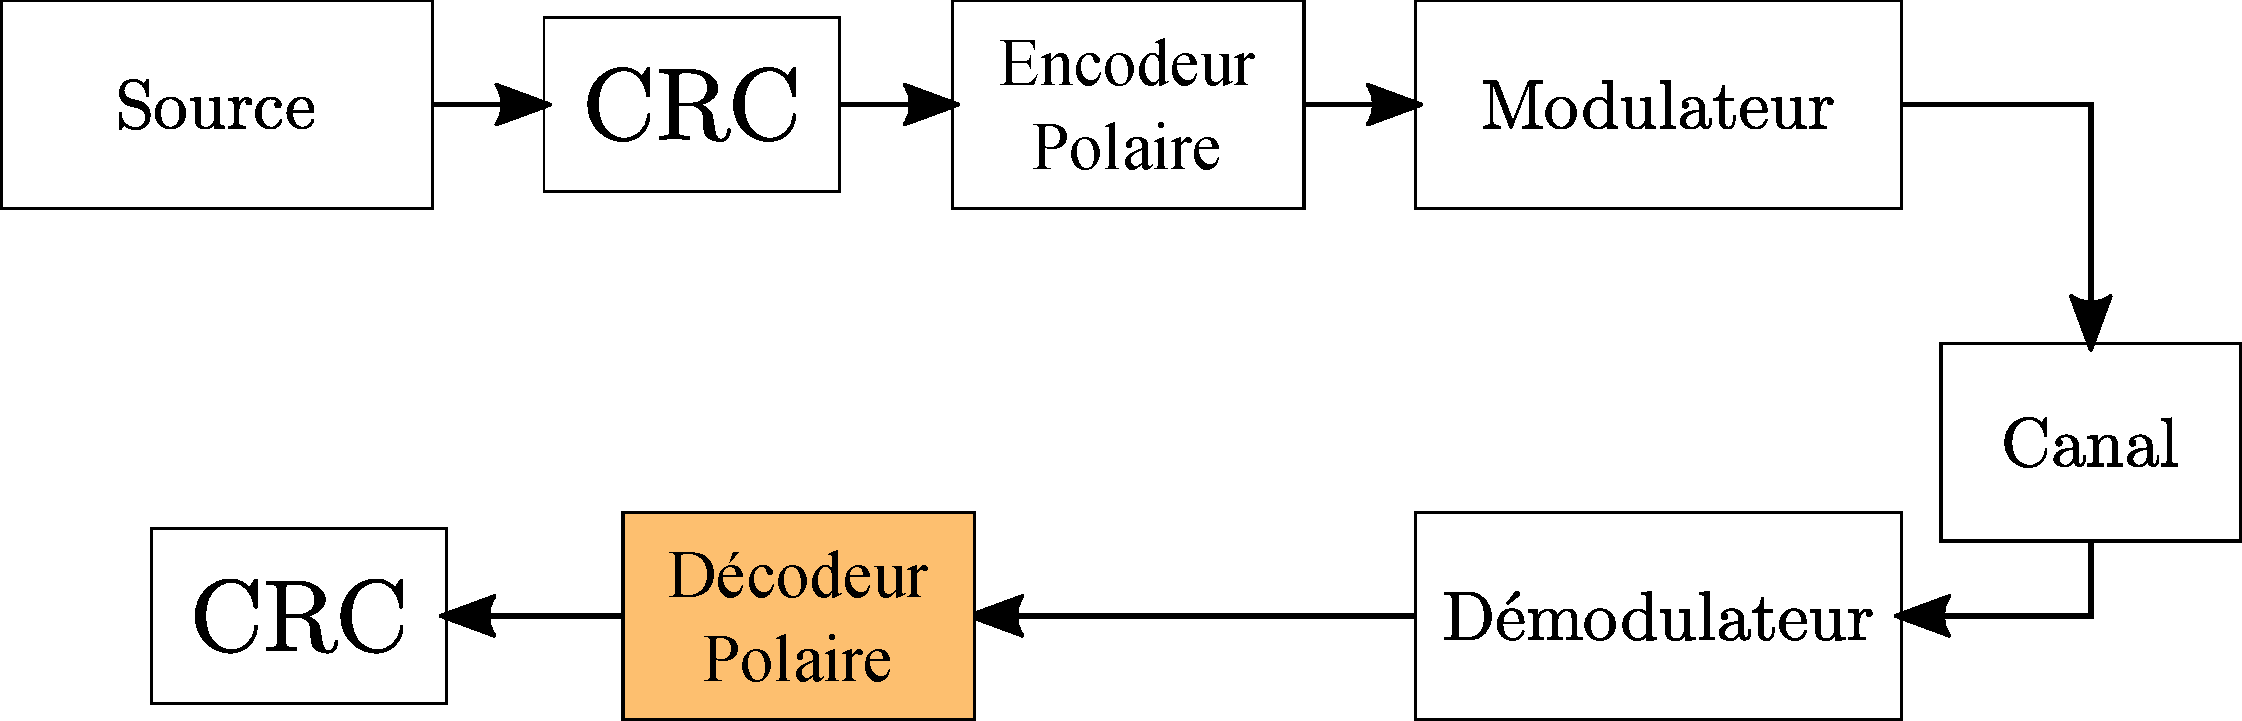
\includegraphics[width=0.7\textwidth]{./fig/extract-1}
  \vfill
\end{frame}

\begin{frame}[c]{Extraction du CRC}
	\centering
  \multiinclude[<+>][start=2,format=pdf,graphics={width=.7\textwidth}]{./fig/extract}

\end{frame}

\begin{frame}[c]{Résumé}
	\begin{itemize}
		\vfill
		\item Les décodeurs logiciels pour les systèmes de communication
		\vfill
		\item Généricité et Flexibilité
		\vfill
		\item Comparaison avec l'état de l'art
		\vfill
		\item Améliorations du débit et de la latence
		\vfill
    \item Mise à disposition du code source \footnote{https://aff3ct.github.io}
    \vfill
	\end{itemize}
\end{frame}

\begin{frame}[c]{Consommation énergétique}

	\begin{minipage}[c][0cm][t]{\textwidth}
	\centering
	\vfill
	\only<1>{Implémentations logicielles sur des processeurs généralistes}
	\vfill
	\only<2>{Implémentations matérielles dédiées}
	\vfill
	\only<3>{Tailles de codes et rendements variés}
	\vfill
	\only<4>{Débits compétitifs des décodeurs logiciels}
	\vfill
	\only<5>{Principal défaut des décodeurs logiciels : la consommation énergétique}
	\vfill
	\only<6>{\GREEN{Comment conserver la flexibilité des décodeurs logiciels en se rapprochant des performances des architectures dédiées ?}}
	\vfill
	\end{minipage}		

	\vspace{1cm}
\centering
	\only<+>{
  \begin{table}[t]
  \begin{tabular}{C{0.9cm}|C{1.9cm}|C{1cm}|C{0.7cm}|C{1.7cm}|C{1.5cm}}
  Ref.           & \textbf{Circuit  } &  N             & R                    & Débit (Mb/s) & $E_b$ (nJ/bit) \\\hline
  \cite{Giard15} & \textbf{i7-4770S  } &  32768        & 0.84                 & 886          & 73             \\
  \cite{6960078} & \textbf{i7-4960HQ } &  32768        & 0.83                 & 1400         & 34             \\
  \cite{7760327} & \textbf{Cortex A57} &  32768        & 0.83                 & 73           & 27             \\\hline
  \cite{6804939} & Stratix IV &  32768                 & 0.9                  & 1200         & -              \\
  \cite{8017407} & ASIC 28nm  &  1024                  & 0.5                  & 94           & 0.095          \\
  \cite{8017407} & ASIC 28nm  &  1024\footnotemark[1]  & 0.5\footnotemark[1]  & 436          & 0.006          \\
  \end{tabular}
  \end{table}
  \footnotetext[1]{\tiny Fixed N \& R}
  }
  \only<+>{
  \begin{table}[t]
  \begin{tabular}{C{0.9cm}|C{1.9cm}|C{1cm}|C{0.7cm}|C{1.7cm}|C{1.5cm}}
	Ref.           & \textbf{Circuit} &  N                     & R                       & Débit (Mb/s) & $E_b$ (nJ/bit)  \\\hline
	\cite{Giard15} & i7-4770S   &  32768                 & 0.84                          & 886        & 73                       \\
	\cite{6960078} & i7-4960HQ  &  32768                 & 0.83                          & 1400       & 34                       \\
	\cite{7760327} & Cortex A57 &  32768                 & 0.83                          & 73         & 27                       \\\hline
	\cite{6804939} & \textbf{Stratix IV} &  32768                 & 0.9                  & 1200       & -               \\
	\cite{8017407} & \textbf{ASIC 28nm } &  1024                  & 0.5                  & 94         & 0.095           \\
	\cite{8017407} & \textbf{ASIC 28nm } &  1024\footnotemark[1]  & 0.5\footnotemark[1]  & 436        & 0.006           \\
	\end{tabular}
  \end{table}

	\footnotetext[1]{\tiny Fixed N \& R}
	}
	\only<+>{
  \begin{table}[t]
  \begin{tabular}{C{0.9cm}|C{1.9cm}|C{1cm}|C{0.7cm}|C{1.7cm}|C{1.5cm}}
	Ref.           & Circuit   &  \textbf{N                  }   & \textbf{R                  }   & Débit (Mb/s) & $E_b$ (nJ/bit)  \\\hline
	\cite{Giard15} & i7-4770S   &  \textbf{32768              }   & \textbf{0.84               }  & 886        & 73              \\
	\cite{6960078} & i7-4960HQ  &  \textbf{32768              }   & \textbf{0.83               }  & 1400       & 34              \\
	\cite{7760327} & Cortex A57 &  \textbf{32768              }   & \textbf{0.83               }  & 73         & 27              \\\hline
	\cite{6804939} & Stratix IV &  \textbf{32768              }   & \textbf{0.9                }  & 1200       & -               \\
	\cite{8017407} & ASIC 28nm  &  \textbf{1024               }   & \textbf{0.5                }  & 94         & 0.095           \\
	\cite{8017407} & ASIC 28nm  &  \textbf{1024\footnotemark[1]}  & \textbf{0.5\footnotemark[1]}  & 436        & 0.006           \\
	\end{tabular}
  \end{table}

	\footnotetext[1]{\tiny Fixed N \& R}
	}

	\only<+>{
  \begin{table}[t]
  \begin{tabular}{C{0.9cm}|C{1.9cm}|C{1cm}|C{0.7cm}|C{1.7cm}|C{1.5cm}}
	Ref.           & Circuit   &  N                     & R                     & \textbf{Débit (Mb/s)} & $E_b$ (nJ/bit)    \\\hline
	\cite{Giard15} & i7-4770S   &  32768                 & 0.84                 & \GREEN{886}        & 73                 \\
	\cite{6960078} & i7-4960HQ  &  32768                 & 0.83                 & \GREEN{1400}       & 34                 \\
	\cite{7760327} & Cortex A57 &  32768                 & 0.83                 & \ORANGE{73}        & 27                 \\\hline
	\cite{6804939} & Stratix IV &  32768                 & 0.9                  & \GREEN{1200}       & -                  \\
	\cite{8017407} & ASIC 28nm  &  1024                  & 0.5                  & \ORANGE{94}        & 0.095              \\
	\cite{8017407} & ASIC 28nm  &  1024\footnotemark[1]  & 0.5\footnotemark[1]  & \GREEN{436}        & 0.006              \\
	\end{tabular}
  \end{table}

	\footnotetext[1]{\tiny Fixed N \& R}
	}
	\only<+>{
  \begin{table}[t]
  \begin{tabular}{C{0.9cm}|C{1.9cm}|C{1cm}|C{0.7cm}|C{1.7cm}|C{1.5cm}}
	Ref.           & Circuit   &  N                     & R                     & Débit (Mb/s) & $\mathbf{E_b}$ \textbf{(nJ/bit)}  \\\hline
	\cite{Giard15} & i7-4770S   &  32768                 & 0.84                 & 886        & \ORANGE{73}                       \\
	\cite{6960078} & i7-4960HQ  &  32768                 & 0.83                 & 1400       & \ORANGE{34}                       \\
	\cite{7760327} & Cortex A57 &  32768                 & 0.83                 & 73         & \ORANGE{27}                       \\\hline
	\cite{6804939} & Stratix IV &  32768                 & 0.9                  & 1200       & \textbf{-}                        \\
	\cite{8017407} & ASIC 28nm  &  1024                  & 0.5                  & 94         & \GREEN{0.095}                     \\
	\cite{8017407} & ASIC 28nm  &  1024\footnotemark[1]  & 0.5\footnotemark[1]  & 436        & \GREEN{0.006}                     \\
	\end{tabular}
  \end{table}

	\footnotetext[1]{\tiny Fixed N \& R}
	}

	\only<+>{
  \begin{table}[t]
	% \vspace{0.5cm}
  \begin{tabular}{C{0.9cm}|C{1.9cm}|C{1cm}|C{0.7cm}|C{1.7cm}|C{1.5cm}}
	Ref.           & Circuit   &  N                     & R                     & Débit (Mb/s) & $E_b$ (nJ/bit)  \\\hline
  \cite{Giard15} & i7-4770S   &  32768                 & 0.84                 & 886        & 73                       \\
  \cite{6960078} & i7-4960HQ  &  32768                 & 0.83                 & 1400       & 34                       \\
  \cite{7760327} & Cortex A57 &  32768                 & 0.83                 & 73         & 27                       \\\hline
  & \GREEN{?} & \GREEN{?} & \GREEN{?} & \GREEN{?} & \GREEN{?}  \\\hline
	\cite{6804939} & Stratix IV &  32768                 & 0.9                  & 1200       & -                        \\
	\cite{8017407} & ASIC 28nm  &  1024                  & 0.5                  & 94         & 0.095                     \\
	\cite{8017407} & ASIC 28nm  &  1024\footnotemark[1]  & 0.5\footnotemark[1]  & 436        & 0.006                     \\
	\end{tabular}
  \end{table}
	}

\end{frame}

%!TEX root = ./soutenance.tex


\section{Conception d'architectures programmables}



\subsection*{Conception d'architectures programmables}


\begin{frame}[c]{Implémentation de l'algorithme SC}
\vfill
  \begin{table}[t]
    \centering
    {\small\resizebox{0.8\linewidth}{!}{
     \begin{tabular}{r|c|c|c} 
      \textbf{Algorithme}  & \textbf{Performances}  & \multirow{2}{*}{\textbf{Débit}} & \textbf{Latence}  \\
      \textbf{de décodage} & \textbf{BER \& FER}    &                                 & \textbf{Maximum}  \\
      \hline
      SC           & \RED{faibles}                  & \GREEN{haut}                    & \GREEN{faible}    \\
      SCL          & \ORANGE{moyennes}              & \RED{bas}                       & \ORANGE{moyenne}  \\
      CA-SCL       & \GREEN{importantes}            & \RED{bas}                       & \ORANGE{moyenne}  \\
      Adaptive-SCL & \GREEN{importantes}            & \GREEN{haut}                    & \RED{forte}       \\
    \end{tabular}
    }}
  \end{table}
  \vfill
  \centering
  L'architecture proposée se concentre sur l'algorithme SC
  \vfill
\end{frame}


\begin{frame}[c]{Deux modèles de conception d'ASIP}
  \centering
  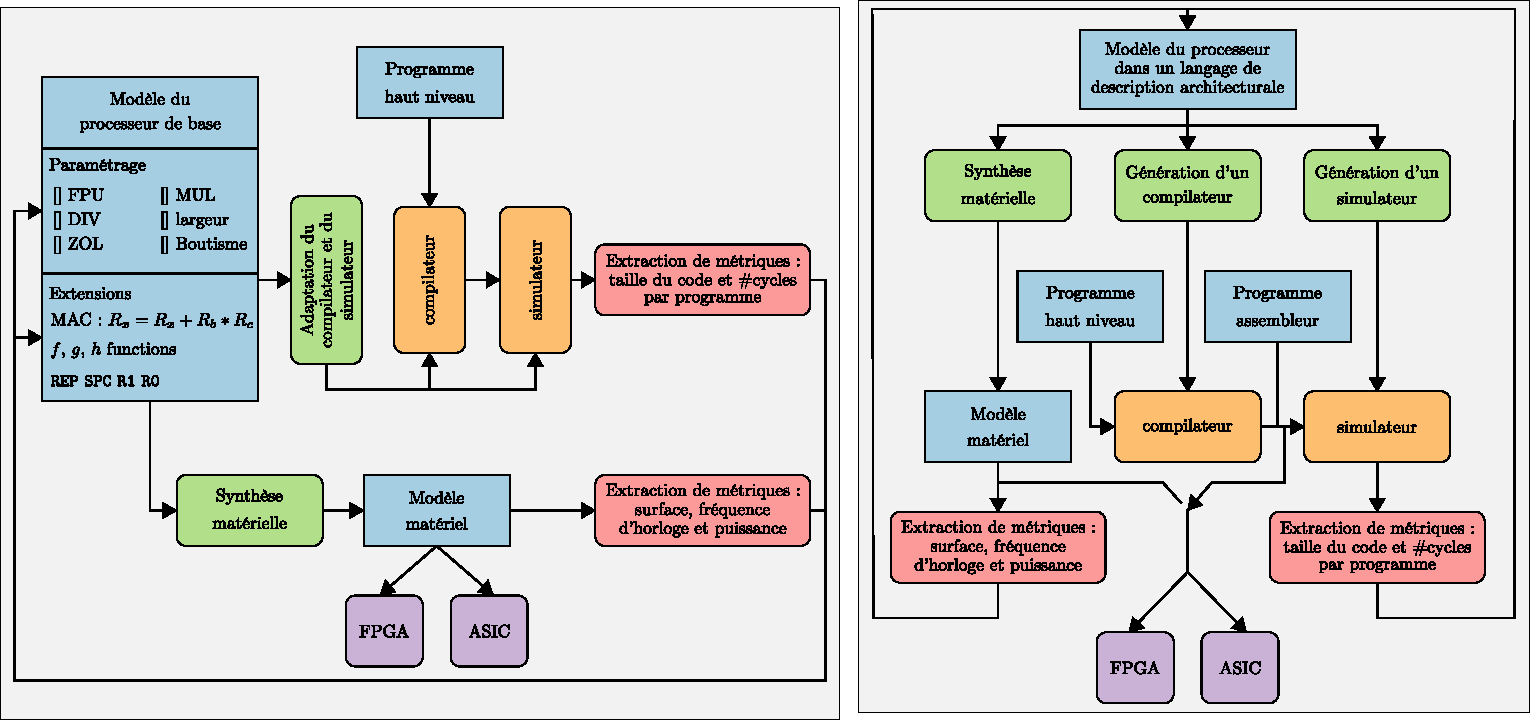
\includegraphics[width=0.9\textwidth]{./fig/methodos}
\end{frame}

\begin{frame}[c]{Approche Tensilica}
\renewcommand{\section}[2]{} % Trick to avoid references section

  \begin{columns}
    \begin{column}{.48\textwidth}
    \vspace{-1cm}
      \begin{itemize}
        \item Spécialisation d'un processeur de base
        \item Instructions spécialisées
        \item Environnement de développement complet
        \item<2-> Réduction de la consommation énergétique
        \item<2-> Publication\color{bluecite}{\cite{leonardon_custom_2018}}
  
      \end{itemize}
    \end{column}
    \begin{column}[T]{.48\textwidth}
    \vspace{-0.5cm}

  \begin{minipage}[c][0cm][t]{\textwidth}
    \only<+>
    { 
      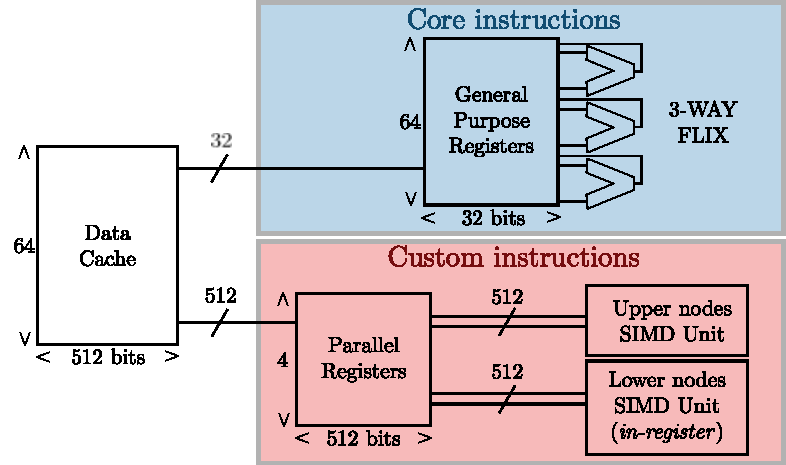
\includegraphics[width=\textwidth]{./fig/archi_tensilica}
    }
    \only<+->
    {
    \begin{table}[t]
      \centering
      {\small\resizebox{\linewidth}{!}{
      \begin{tabular}{c|c|c|c|c}
        \toprule

        Target & $N$ & \begin{tabular}{c}Latency\\{[$\mu$s]}\end{tabular} & \begin{tabular}{c}Throughput\\{[Mb/s]}\end{tabular} & \begin{tabular}{c}$E_b$\\{[nJ]}\end{tabular} \\

        \cmidrule(lr){1-1}
        \cmidrule(lr){2-2}
        \cmidrule(lr){3-5}
%                       
        \multirow{4}{*}{\bf A57-1.1GHz}  & $1024$   & $13$  & $38$  & \ORANGE{$\mathbf{21}$} \\

                                         & $512$    & $6.7$ & $38$  & \ORANGE{$\mathbf{21}$} \\

                                         & $256$    & $3.6$ & $35$  & \ORANGE{$\mathbf{22}$}\\

                                         & $128$    & $2.1$ & $30$  & \ORANGE{$\mathbf{27}$}\\

        \midrule

        \multirow{4}{*}{\bf i7-3.3GHz}   & $1024$   & $2.3$ & $222$ & \RED{$\mathbf{47}$} \\

                                         & $512$    & $1.4$ & $182$ & \RED{$\mathbf{57}$} \\

                                         & $256$    & $0.8$ & $155$ & \RED{$\mathbf{68}$}\\

                                         & $128$    & $0.5$ & $124$ & \RED{$\mathbf{85}$}\\

        \midrule

        \multirow{4}{*}{\bf ASIP-835MHz} & $1024$   & $7.2$ & $71$  & \GREEN{$\mathbf{1.6}$} \\

                                         & $512$    & $3.9$ & $66$  & \GREEN{$\mathbf{1.7}$} \\

                                         & $256$    & $1.9$ & $65$  & \GREEN{$\mathbf{1.7}$}\\

                                         & $128$    & $1.0$ & $62$  & \GREEN{$\mathbf{1.8}$}\\
        \bottomrule
      \end{tabular}
      }}
    \end{table}
    }
  \end{minipage} 
    \end{column}
  \end{columns}
\vfill
\centering
  \begin{minipage}[c][0cm][t]{\textwidth}
\only<2>
{
    \printbibliography[keyword={leonardon}]

}
  \end{minipage} 
\end{frame}


\begin{frame}[c]{Limites de l'approche Tensilica}
  \begin{itemize}
    \vfill
    \item Limitation de l'accès à la mémoire
    \vfill
    \item Rigidité de l'architecture
    \vfill
    \item Langage de description matérielle spécifique
    \vfill
    \item Licence nécessaire
    \vfill
  \end{itemize}
\end{frame}

\begin{frame}[c]{Transport Triggered Architectures}
  \begin{itemize}
    \vfill
    \item Modèle de processeur
    \vfill
    \item Similaire aux architectures VLIW
    \vfill
    \item Parallélisme de données
    \vfill
    \item Parallélisme d'instructions
    \vfill
  \end{itemize}
\end{frame}

\begin{frame}[c]{Structure d'un processeur TTA}
  \multiinclude[<+>][start=1,format=pdf,graphics={width=.8\textwidth}]{./fig/anim_tta_base}
\end{frame}

\begin{frame}[c]{Niveau de parallélisme}
  Two main polar functions : $f$ and $g$
  \vspace{1cm}

  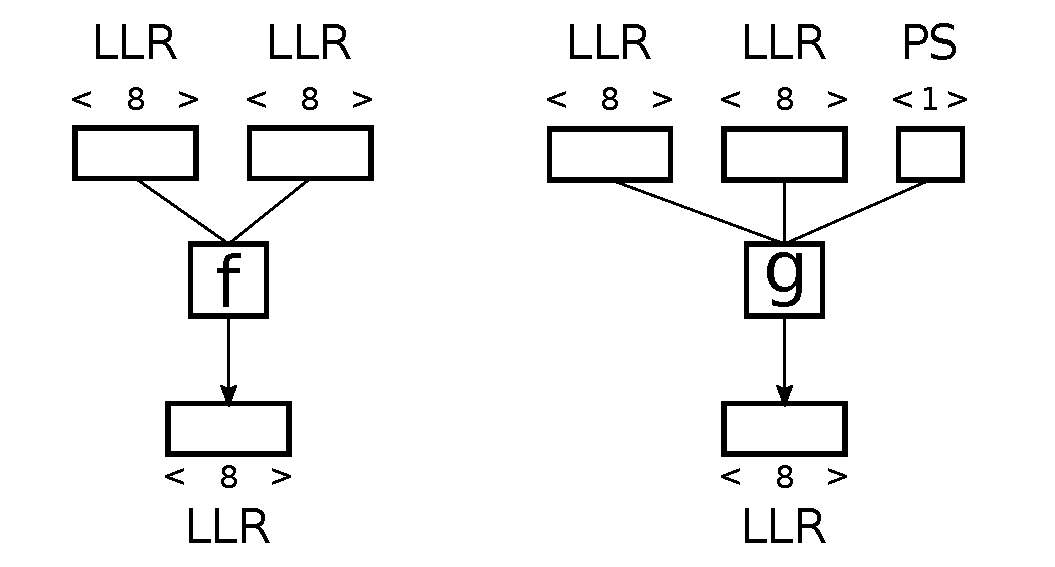
\includegraphics[width=0.7\textwidth]{fig/f_g_dimensions_scalar}
\end{frame}

\begin{frame}[c]{Niveau de parallélisme}
  Two main polar functions : $f$ and $g$
  \vspace{1cm}

  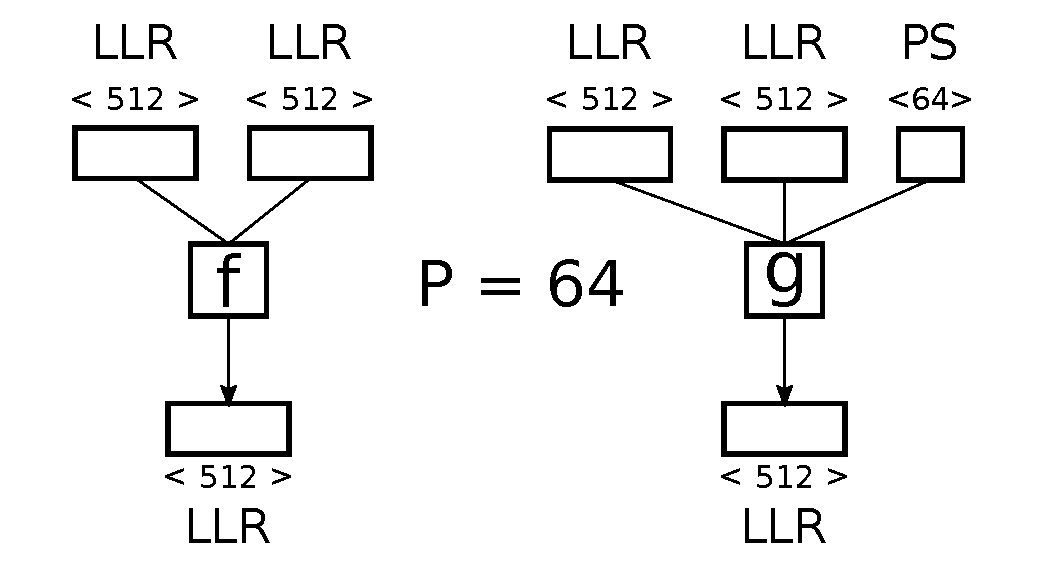
\includegraphics[width=0.7\textwidth]{fig/f_g_dimensions_vector}
\end{frame}

\begin{frame}[c]{Conception du processeur}
  \begin{columns}[T] % align columns
    \begin{column}{.48\textwidth}
      \vspace{-0.5cm}
      \multiinclude[<+>][start=1,format=pdf,graphics={width=1.4\textwidth}]{./fig/archi_sc_construction}
    \end{column}
    \begin{column}{.07\textwidth}
    \end{column}
    \begin{column}{.41\textwidth}
      \begin{itemize}
        \item<1-> Mémoires vectorielles
        \vspace{0.2cm}
        \item<2-> 2 bus de 512 bits
        \vspace{0.2cm}
        \item<2-> 1 bus de 64 bits
        \vspace{0.2cm}
        \item<3-> Unité de chargement et sauvegarde vectorielles
        \vspace{0.2cm}
        \item<4-> Unité de calcul polaire
      \end{itemize}
    \end{column}
  \end{columns} % align columns
\end{frame}

\begin{frame}[c]{Compilation}
  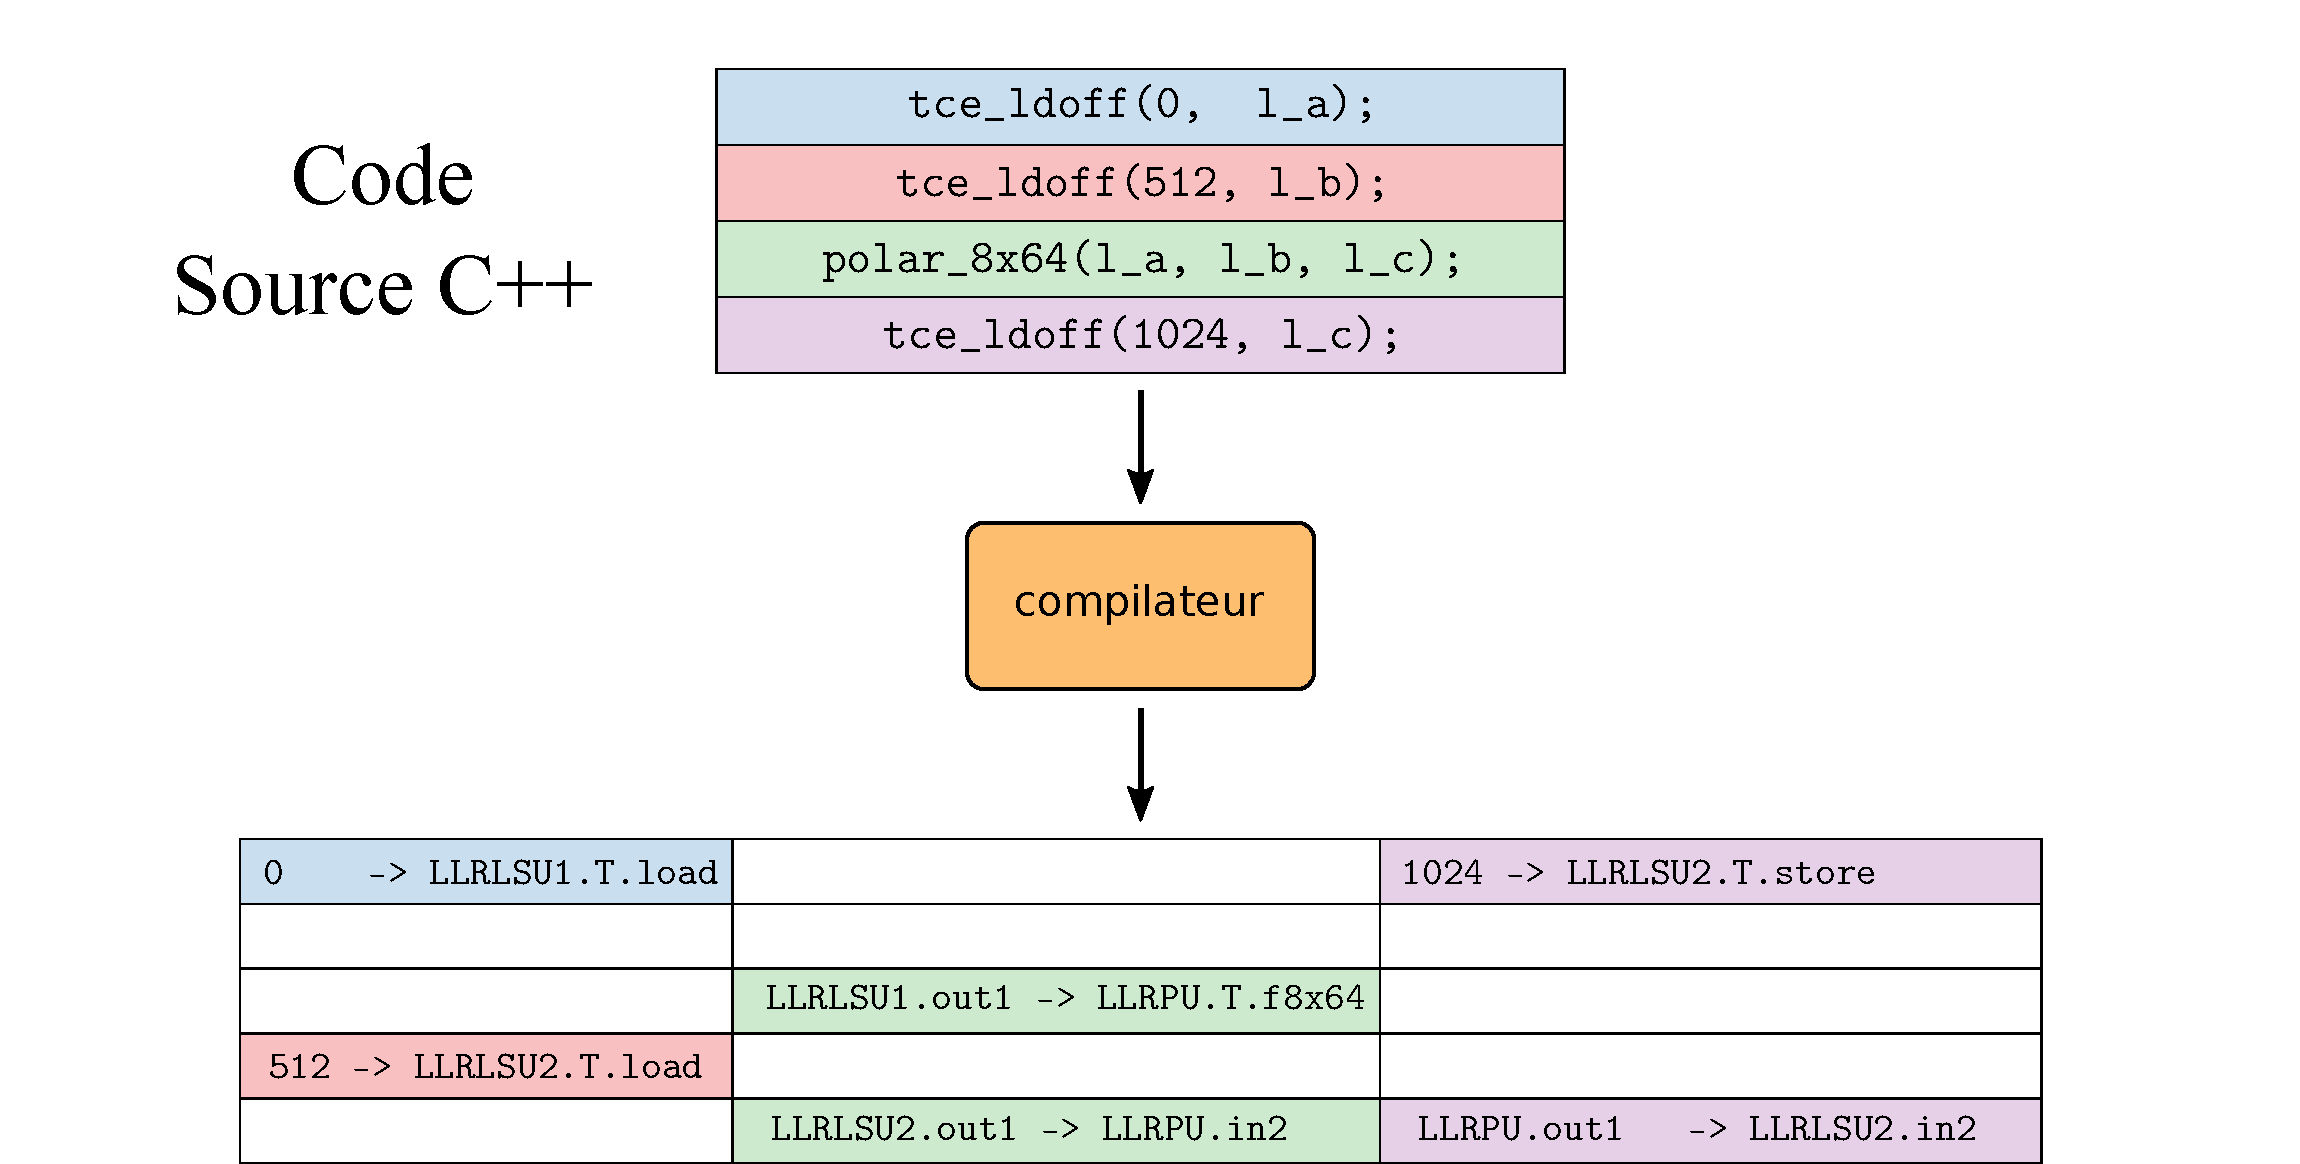
\includegraphics[width=\textwidth]{fig/compilation}
\end{frame}

\begin{frame}[c]{Parallélisme d'instruction}
  \multiinclude[<+>][start=1,format=pdf,graphics={width=.8\textwidth}]{./fig/ilp}
\end{frame}





\begin{frame}[c]{Comparaison avec des décodeurs logiciels}
  \begin{columns}[T] % align columns
  \begin{column}{.48\textwidth}
    \begin{itemize}
      \item<+-> Architecture proposée
      \item<+-> Processeurs Intel x86 (i7-4712HQ) et ARM (Cortex A57)
      \begin{itemize}
        \item<+-> Boîte à outils logicielle \textbf{AFF3CT}
        \item<+-> SIMD (Neon \& AVX2)
      \end{itemize}
      \item<+-> ASIP de type Tensilica
      \item<+-> Débit meximum atteint par le processeur proposé
      \item<+-> Consommation énergétique réduite d'un à deux ordres de grandeur
    \end{itemize}
  \end{column}

  \begin{column}{.48\textwidth}
  \only<1>{
    \begin{table}
      \centering
      {
      \small\resizebox{\linewidth}{!}{
      \begin{tabular}{c|c|c|c|c}
        \toprule

        Architecture & $N$ & \begin{tabular}{c}Latence\\{[$\mu$s]}\end{tabular} & \begin{tabular}{c}Débit\\{[Mb/s]}\end{tabular} & \begin{tabular}{c}$E_b$\\{[nJ/bit]}\end{tabular} \\

        \cmidrule(lr){1-1}
        \cmidrule(lr){2-2}
        \cmidrule(lr){3-5}

        \multirow{2}{*}{\bf \BLUE{TTPD-800MHz}}     & $1024$   & $1.4$  & $352$ & $0.14$ \\ % 1512 cycles
                                                    & $512$    & $0.8$  & $313$ & $0.15$ \\ % 803 cycles
        \multirow{2}{*}{\bf \BLUE{(ASIP)}}          & $256$    & $0.4$  & $304$ & $0.16$ \\ % 413 cycles
                                                    & $128$    & $0.2$  & $284$ & $0.17$ \\ % 224 cycles
        \midrule
        \multirow{2}{*}{\bf i7-3.3GHz}              & $1024$   & $2.0$  & $257$ & $41$   \\
                                                    & $512$    & $1.2$  & $210$ & $49$   \\
        \multirow{2}{*}{\bf (GPP)}                  & $256$    & $0.7$  & $179$ & $59$   \\
                                                    & $128$    & $0.4$  & $143$ & $73$   \\
        \midrule    
        \multirow{2}{*}{\bf A57-1.1GHz}             & $1024$   & $10.7$ & $48$  & $17$   \\
                                                    & $512$    & $5.3$  & $48$  & $17$   \\
        \multirow{2}{*}{\bf (GPP)}                  & $256$    & $2.8$  & $46$  & $17$   \\
                                                    & $128$    & $1.6$  & $41$  & $20$   \\
        \midrule
        \multirow{2}{*}{\bf LX7-835MHz}             & $1024$   & $7.2$  & $71$  & $1.6$  \\
                                                    & $512$    & $3.9$  & $66$  & $1.7$  \\
        \multirow{2}{*}{\bf (ASIP)}                 & $256$    & $1.9$  & $65$  & $1.7$  \\
                                                    & $128$    & $1.0$  & $62$  & $1.8$  \\
        \bottomrule
      \end{tabular}
      }}
    \end{table}
  }
    
    \only<2-4>{
    \begin{table}
      \centering
      {
      \small\resizebox{\linewidth}{!}{
      \begin{tabular}{c|c|c|c|c}
        \toprule

        Architecture & $N$ & \begin{tabular}{c}Latence\\{[$\mu$s]}\end{tabular} & \begin{tabular}{c}Débit\\{[Mb/s]}\end{tabular} & \begin{tabular}{c}$E_b$\\{[nJ/bit]}\end{tabular} \\

        \cmidrule(lr){1-1}
        \cmidrule(lr){2-2}
        \cmidrule(lr){3-5}


        \multirow{2}{*}{\bf TTPD-800MHz}            & $1024$   & $1.4$  & $352$ & $0.14$ \\ % 1512 cycles
                                                    & $512$    & $0.8$  & $313$ & $0.15$ \\ % 803 cycles
        \multirow{2}{*}{\bf (ASIP)}                 & $256$    & $0.4$  & $304$ & $0.16$ \\ % 413 cycles
                                                    & $128$    & $0.2$  & $284$ & $0.17$ \\ % 224 cycles
        \midrule
        \multirow{2}{*}{\bf \BLUE{i7-3.3GHz}}       & $1024$   & $2.0$  & $257$ & $41$   \\
                                                    & $512$    & $1.2$  & $210$ & $49$   \\
        \multirow{2}{*}{\bf \BLUE{(GPP)}}           & $256$    & $0.7$  & $179$ & $59$   \\
                                                    & $128$    & $0.4$  & $143$ & $73$   \\
        \midrule    
        \multirow{2}{*}{\bf \BLUE{A57-1.1GHz}}      & $1024$   & $10.7$ & $48$  & $17$   \\
                                                    & $512$    & $5.3$  & $48$  & $17$   \\
        \multirow{2}{*}{\bf \BLUE{(GPP)}}           & $256$    & $2.8$  & $46$  & $17$   \\
                                                    & $128$    & $1.6$  & $41$  & $20$   \\
        \midrule
        \multirow{2}{*}{\bf LX7-835MHz}             & $1024$   & $7.2$  & $71$  & $1.6$  \\
                                                    & $512$    & $3.9$  & $66$  & $1.7$  \\
        \multirow{2}{*}{\bf (ASIP)}                 & $256$    & $1.9$  & $65$  & $1.7$  \\
                                                    & $128$    & $1.0$  & $62$  & $1.8$  \\
        \bottomrule
      \end{tabular}
      }}
    \end{table}
    }

  \only<5>{
    \begin{table}
      \centering
      {
      \small\resizebox{\linewidth}{!}{
      \begin{tabular}{c|c|c|c|c}
        \toprule

        Architecture & $N$ & \begin{tabular}{c}Latence\\{[$\mu$s]}\end{tabular} & \begin{tabular}{c}Débit\\{[Mb/s]}\end{tabular} & \begin{tabular}{c}$E_b$\\{[nJ/bit]}\end{tabular} \\

        \cmidrule(lr){1-1}
        \cmidrule(lr){2-2}
        \cmidrule(lr){3-5}


        \multirow{2}{*}{\bf TTPD-800MHz}            & $1024$   & $1.4$  & $352$ & $0.14$ \\ % 1512 cycles
                                                    & $512$    & $0.8$  & $313$ & $0.15$ \\ % 803 cycles
        \multirow{2}{*}{\bf (ASIP)}                 & $256$    & $0.4$  & $304$ & $0.16$ \\ % 413 cycles
                                                    & $128$    & $0.2$  & $284$ & $0.17$ \\ % 224 cycles
        \midrule
        \multirow{2}{*}{\bf i7-3.3GHz}              & $1024$   & $2.0$  & $257$ & $41$   \\
                                                    & $512$    & $1.2$  & $210$ & $49$   \\
        \multirow{2}{*}{\bf (GPP)}                  & $256$    & $0.7$  & $179$ & $59$   \\
                                                    & $128$    & $0.4$  & $143$ & $73$   \\
        \midrule    
        \multirow{2}{*}{\bf A57-1.1GHz}             & $1024$   & $10.7$ & $48$  & $17$   \\
                                                    & $512$    & $5.3$  & $48$  & $17$   \\
        \multirow{2}{*}{\bf (GPP)}                  & $256$    & $2.8$  & $46$  & $17$   \\
                                                    & $128$    & $1.6$  & $41$  & $20$   \\
        \midrule
        \multirow{2}{*}{\bf \BLUE{LX7-835MHz}}      & $1024$   & $7.2$  & $71$  & $1.6$  \\
                                                    & $512$    & $3.9$  & $66$  & $1.7$  \\
        \multirow{2}{*}{\bf \BLUE{(ASIP)}}          & $256$    & $1.9$  & $65$  & $1.7$  \\
                                                    & $128$    & $1.0$  & $62$  & $1.8$  \\

        \bottomrule
      \end{tabular}
      }}
    \end{table}
    }
    \only<6>{
    \begin{table}
      \centering
      {
      \small\resizebox{\linewidth}{!}{
      \begin{tabular}{c|c|c|c|c}
        \toprule

        Architecture & $N$ & \begin{tabular}{c}Latence\\{[$\mu$s]}\end{tabular} & \begin{tabular}{c}Débit\\{[Mb/s]}\end{tabular} & \begin{tabular}{c}$E_b$\\{[nJ/bit]}\end{tabular} \\

        \cmidrule(lr){1-1}
        \cmidrule(lr){2-2}
        \cmidrule(lr){3-5}


        \multirow{2}{*}{\bf TTPD-800MHz}            & $1024$   & $1.4$  & \GREEN{$\mathbf{352}$} & $0.14$ \\ % 1512 cycles
                                                    & $512$    & $0.8$  & \GREEN{$\mathbf{313}$} & $0.15$ \\ % 803 cycles
        \multirow{2}{*}{\bf (ASIP)}                 & $256$    & $0.4$  & \GREEN{$\mathbf{304}$} & $0.16$ \\ % 413 cycles
                                                    & $128$    & $0.2$  & \GREEN{$\mathbf{284}$} & $0.17$ \\ % 224 cycles
        \midrule
        \multirow{2}{*}{\bf i7-3.3GHz}              & $1024$   & $2.0$  & \GREEN{$\mathbf{257}$} & $41$   \\
                                                    & $512$    & $1.2$  & \GREEN{$\mathbf{210}$} & $49$   \\
        \multirow{2}{*}{\bf (GPP)}                  & $256$    & $0.7$  & \GREEN{$\mathbf{179}$} & $59$   \\
                                                    & $128$    & $0.4$  & \GREEN{$\mathbf{143}$} & $73$   \\
        \midrule    
        \multirow{2}{*}{\bf A57-1.1GHz}             & $1024$   & $10.7$ & \ORANGE{$\mathbf{48}$} & $17$   \\
                                                    & $512$    & $5.3$  & \ORANGE{$\mathbf{48}$} & $17$   \\
        \multirow{2}{*}{\bf (GPP)}                  & $256$    & $2.8$  & \ORANGE{$\mathbf{46}$} & $17$   \\
                                                    & $128$    & $1.6$  & \ORANGE{$\mathbf{41}$} & $20$   \\
        \midrule
        \multirow{2}{*}{\bf LX7-835MHz}             & $1024$   & $7.2$  & \ORANGE{$\mathbf{71}$} & $1.6$  \\
                                                    & $512$    & $3.9$  & \ORANGE{$\mathbf{66}$} & $1.7$  \\
        \multirow{2}{*}{\bf (ASIP)}                 & $256$    & $1.9$  & \ORANGE{$\mathbf{65}$} & $1.7$  \\
                                                    & $128$    & $1.0$  & \ORANGE{$\mathbf{62}$} & $1.8$  \\

        \bottomrule
      \end{tabular}
      }}
    \end{table}
    }
    \only<7>{
    \begin{table}
      \centering
      {
      \small\resizebox{\linewidth}{!}{
      \begin{tabular}{c|c|c|c|c}
        \toprule

        Architecture & $N$ & \begin{tabular}{c}Latence\\{[$\mu$s]}\end{tabular} & \begin{tabular}{c}Débit\\{[Mb/s]}\end{tabular} & \begin{tabular}{c}$E_b$\\{[nJ/bit]}\end{tabular} \\

        \cmidrule(lr){1-1}
        \cmidrule(lr){2-2}
        \cmidrule(lr){3-5}


        \multirow{2}{*}{\bf TTPD-800MHz}            & $1024$   & $1.4$  & $352$ & \GREEN{$\mathbf{0.14}$} \\ % 1512 cycles
                                                    & $512$    & $0.8$  & $313$ & \GREEN{$\mathbf{0.15}$} \\ % 803 cycles
        \multirow{2}{*}{\bf (ASIP)}                 & $256$    & $0.4$  & $304$ & \GREEN{$\mathbf{0.16}$} \\ % 413 cycles
                                                    & $128$    & $0.2$  & $284$ & \GREEN{$\mathbf{0.17}$} \\ % 224 cycles
        \midrule
        \multirow{2}{*}{\bf i7-3.3GHz}              & $1024$   & $2.0$  & $257$ & \RED{$\mathbf{41}$}   \\
                                                    & $512$    & $1.2$  & $210$ & \RED{$\mathbf{49}$}   \\
        \multirow{2}{*}{\bf (GPP)}                  & $256$    & $0.7$  & $179$ & \RED{$\mathbf{59}$}   \\
                                                    & $128$    & $0.4$  & $143$ & \RED{$\mathbf{73}$}   \\
        \midrule    
        \multirow{2}{*}{\bf A57-1.1GHz}             & $1024$   & $10.7$ & $48$  & \RED{$\mathbf{17}$}   \\
                                                    & $512$    & $5.3$  & $48$  & \RED{$\mathbf{17}$}   \\
        \multirow{2}{*}{\bf (GPP)}                  & $256$    & $2.8$  & $46$  & \RED{$\mathbf{17}$}   \\
                                                    & $128$    & $1.6$  & $41$  & \RED{$\mathbf{20}$}   \\
        \midrule
        \multirow{2}{*}{\bf LX7-835MHz}             & $1024$   & $7.2$  & $71$  & \ORANGE{$\mathbf{1.6}$}  \\
                                                    & $512$    & $3.9$  & $66$  & \ORANGE{$\mathbf{1.7}$}  \\
        \multirow{2}{*}{\bf (ASIP)}                 & $256$    & $1.9$  & $65$  & \ORANGE{$\mathbf{1.7}$}  \\
                                                    & $128$    & $1.0$  & $62$  & \ORANGE{$\mathbf{1.8}$}  \\

        \bottomrule
      \end{tabular}
      }}
    \end{table}
    }
  \end{column}
  \end{columns}
\end{frame}


\begin{frame}[c]{Comparaison avec des architectures matérielles dédiées}
    \begin{itemize}
      \item<+-> Processeur proposé
      \item<+-> Décodeur matériel dédié
      \item<2-> Décodeur matériel dédié avec construction optimisée
      \item<+-> Implémentations FPGA
    \end{itemize}

    \only<1>{
      \begin{table}
      \centering
      {
        \small\resizebox{0.8\linewidth}{!}{
        \begin{tabular}{c|c|c|c|c}
                                  & \BLUE{TTPD Proposé}  & \cite{giard_638_2015} & \multicolumn{2}{c}{\cite{sarkis2014fast}} \\
          \cmidrule(lr){2-2}
          \cmidrule(lr){3-3}
          \cmidrule(lr){4-5}

          \textbf{FPGA}               &  Artix 7       & Stratix IV            & Stratix IV         & Virtex 6             \\
          \textbf{Cycles d'horloge}   &  1161          & 222                   & 165                & 165                  \\
          \textbf{\'Elagage}          &  R0 \& R1      & Complet               & Complet            & Complet              \\
          \textbf{LUTS}               &  14744         & 23020                 & 24821              & 22115                \\
          \textbf{RAM} (Kb)           &  141           & 43                    & 36                 & 36                   \\

        \end{tabular}
      }}
      \end{table}
    }

    \only<2>{
      \begin{table}
      \centering
      {
        \small\resizebox{0.8\linewidth}{!}{
        \begin{tabular}{c|c|c|c|c}
                                  & TTPD Proposé  & \BLUE{\cite{giard_638_2015}} & \multicolumn{2}{c}{\BLUE{\cite{sarkis2014fast}}} \\
          \cmidrule(lr){2-2}
          \cmidrule(lr){3-3}
          \cmidrule(lr){4-5}

          \textbf{FPGA}         &  Artix 7       & Stratix IV            & Stratix IV         & Virtex 6             \\
          \textbf{Cycles d'horloge}   &  1161          & 222                   & 165                & 165                  \\
          \textbf{\'Elagage}        &  R0 \& R1      & Complet                  & Complet               & Complet                 \\
          \textbf{LUTS}           &  14744         & 23020                 & 24821              & 22115                \\
          \textbf{RAM} (Kb)       &  141           & 43                    & 36                 & 36                   \\

        \end{tabular}
      }}
      \end{table}
    }

    \only<3>{
      \begin{table}
      \centering
      {
        \small\resizebox{0.8\linewidth}{!}{
        \begin{tabular}{c|c|c|c|c}
                                  & TTPD Proposé  & \cite{giard_638_2015} & \multicolumn{2}{c}{\cite{sarkis2014fast}} \\
          \cmidrule(lr){2-2}
          \cmidrule(lr){3-3}
          \cmidrule(lr){4-5}

          \textbf{FPGA}         &  \textbf{Artix 7}       & \textbf{Stratix IV}            & \textbf{Stratix IV }        & \textbf{Virtex 6}             \\
          \textbf{Cycles d'horloge}   &  1161          & 222                   & 165                & 165                  \\
          \textbf{\'Elagage}        &  R0 \& R1      & Complet                  & Complet               & Complet                 \\
          \textbf{LUTS}           &  14744         & 23020                 & 24821              & 22115                \\
          \textbf{RAM} (Kb)       &  141           & 43                    & 36                 & 36                   \\

        \end{tabular}
      }}
      \end{table}
    }
\end{frame}

\begin{frame}[c]{Comparaison avec des architectures matérielles dédiées}
    \begin{itemize}
      \item<+-> 5 à six fois plus de cycles
      \item<+-> Différents niveaux d'élagage
      \item<+-> Plus petit nombre de LUTs
      \item<+-> Plus grosse empreinte mémoire
    \end{itemize}

    \only<1>{
      \begin{table}
      \centering
      {
        \small\resizebox{0.8\linewidth}{!}{
        \begin{tabular}{c|c|c|c|c}
                                  & TTPD Proposé  & \cite{giard_638_2015} & \multicolumn{2}{c}{\cite{sarkis2014fast}} \\
          \cmidrule(lr){2-2}
          \cmidrule(lr){3-3}
          \cmidrule(lr){4-5}

          \textbf{FPGA}         &  Artix 7       & Stratix IV            & Stratix IV         & Virtex 6             \\
          \textbf{Cycles d'horloge}   &  \textbf{1161}  & \textbf{222}           & \textbf{165}        & \textbf{165}          \\
          \textbf{\'Elagage}        &  R0 \& R1      & Complet                  & Complet               & Complet                 \\
          \textbf{LUTS}           &  14744         & 23020                 & 24821              & 22115                \\
          \textbf{RAM} (Kb)       &  141           & 43                    & 36                 & 36                   \\

        \end{tabular}
      }}
      \end{table}
    }
    \only<2>{
      \begin{table}
      \centering
      {
        \small\resizebox{0.8\linewidth}{!}{
        \begin{tabular}{c|c|c|c|c}
                                  & TTPD Proposé  & \cite{giard_638_2015} & \multicolumn{2}{c}{\cite{sarkis2014fast}} \\
          \cmidrule(lr){2-2}
          \cmidrule(lr){3-3}
          \cmidrule(lr){4-5}

          \textbf{FPGA}         &  Artix 7       & Stratix IV            & Stratix IV         & Virtex 6             \\
          \textbf{Cycles d'horloge}   &  1161          & 222                   & 165                & 165                  \\
          \textbf{\'Elagage}        &  \textbf{R0 \& R1}      & \textbf{Complet}                  & \textbf{Complet}               & \textbf{Complet}                 \\
          \textbf{LUTS}           &  14744         & 23020                 & 24821              & 22115                \\
          \textbf{RAM} (Kb)       &  141           & 43                    & 36                 & 36                   \\

        \end{tabular}
      }}
      \end{table}
    }
    \only<3>{
      \begin{table}
      \centering
      {
        \small\resizebox{0.8\linewidth}{!}{
        \begin{tabular}{c|c|c|c|c}
                                  & TTPD Proposé  & \cite{giard_638_2015} & \multicolumn{2}{c}{\cite{sarkis2014fast}} \\
          \cmidrule(lr){2-2}
          \cmidrule(lr){3-3}
          \cmidrule(lr){4-5}

          \textbf{FPGA}         &  Artix 7        & Stratix IV             & Stratix IV          & Virtex 6              \\
          \textbf{Cycles d'horloge}   &  1161           & 222                    & 165                 & 165                   \\
          \textbf{\'Elagage}        &  R0 \& R1       & Complet                   & Complet                & Complet                  \\
          \textbf{LUTS}           &  \textbf{14744} & \textbf{23020}         & \textbf{24821}      & \textbf{22115}        \\
          \textbf{RAM} (Kb)       &  141            & 43                     & 36                  & 36                    \\


        \end{tabular}
      }}
      \end{table}
    }
    \only<4>{
      \begin{table}
      \centering
      {
        \small\resizebox{0.8\linewidth}{!}{
        \begin{tabular}{c|c|c|c|c}
                                  & TTPD Proposé  & \cite{giard_638_2015} & \multicolumn{2}{c}{\cite{sarkis2014fast}} \\
          \cmidrule(lr){2-2}
          \cmidrule(lr){3-3}
          \cmidrule(lr){4-5}

          \textbf{FPGA}         &  Artix 7       & Stratix IV            & Stratix IV         & Virtex 6             \\
          \textbf{Cycles d'horloge}   &  1161          & 222                   & 165                & 165                  \\
          \textbf{\'Elagage}        &  R0 \& R1      & Complet                  & Complet               & Complet                  \\
          \textbf{LUTS}           &  14744         & 23020                 & 24821              & 22115                \\
          \textbf{RAM} (Kb)       &  \textbf{141}  & \textbf{43}           & \textbf{36}        & \textbf{36}          \\


        \end{tabular}
      }}
      \end{table}
    }
\end{frame}

\section{Conclusions et perspectives}
\subsection*{}

\begin{frame}[c]{Conclusions}

  \begin{enumerate}
\renewcommand{\section}[2]{} % Trick to avoid references section

    \renewcommand*{\bibfont}{\scriptsize}
    \nocite{leonardon_fast_2017,ghaffari_improving_2017,leonardon_tta_2018,Ghaffari2018,cassagne_fast_2017,cassagne_gdr_2017}
    \vfill
    \item<+-> Implémentation logicielle de l'algorithme  SCL
    \scriptsize{\printbibliography[keyword={fast-scl}]}
    \vfill
    \item<+-> Spécialisation d'un processeur Tensilica
    \scriptsize{\printbibliography[keyword={leonardon}]}
    \vfill
    \item<+-> Conception d'un processeur de type TTA
    \scriptsize{\printbibliography[keyword={tta}]}
    \vfill
    \item<+-> Implémentation du décodeur SCMA
    \printbibliography[keyword={ghaffari}]
    \vfill
    \item<+-> Participation au projet AFF3CT
    \printbibliography[keyword={aff3ct}]
    \vfill
  \end{enumerate}

\end{frame}

\begin{frame}[c]{Perspectives}

  \begin{itemize}
    \renewcommand*{\bibfont}{\scriptsize}
    \vfill
    \item<+-> Extension des travaux sur les décodeurs logiciels
    \begin{itemize}
      \item Implémentations logicielles des algorithmes SCF, SCS
      \item Support des codes polaires multinoyaux
    \end{itemize}
    \vfill
    \item<+-> Architecture TTA supportant le décodage de l'algorithme SCL
    \vfill
    \item<+-> Intégration des codes polaires dans des chaînes de communications plus complexes
    \begin{itemize}
      \item Travaux sur le SCMA
      \item Support des codes polaires de la 5G
    \end{itemize}
    \vfill
  \end{itemize}

\end{frame}

\begin{frame}[c]{Merci}
\vfill
Merci pour votre attention !
\vfill
\end{frame}

\begin{frame}[allowframebreaks]{References}
\renewcommand*{\bibfont}{\scriptsize}

\printbibliography
\end{frame}


\end{document}

